\documentclass[12pt]{article}
\usepackage{graphicx}
\usepackage{fullpage}
\usepackage{amsmath,enumerate,here}
\usepackage{gensymb}



\begin{document}

\section{Main Figures}


\begin{figure}
\begin{center}
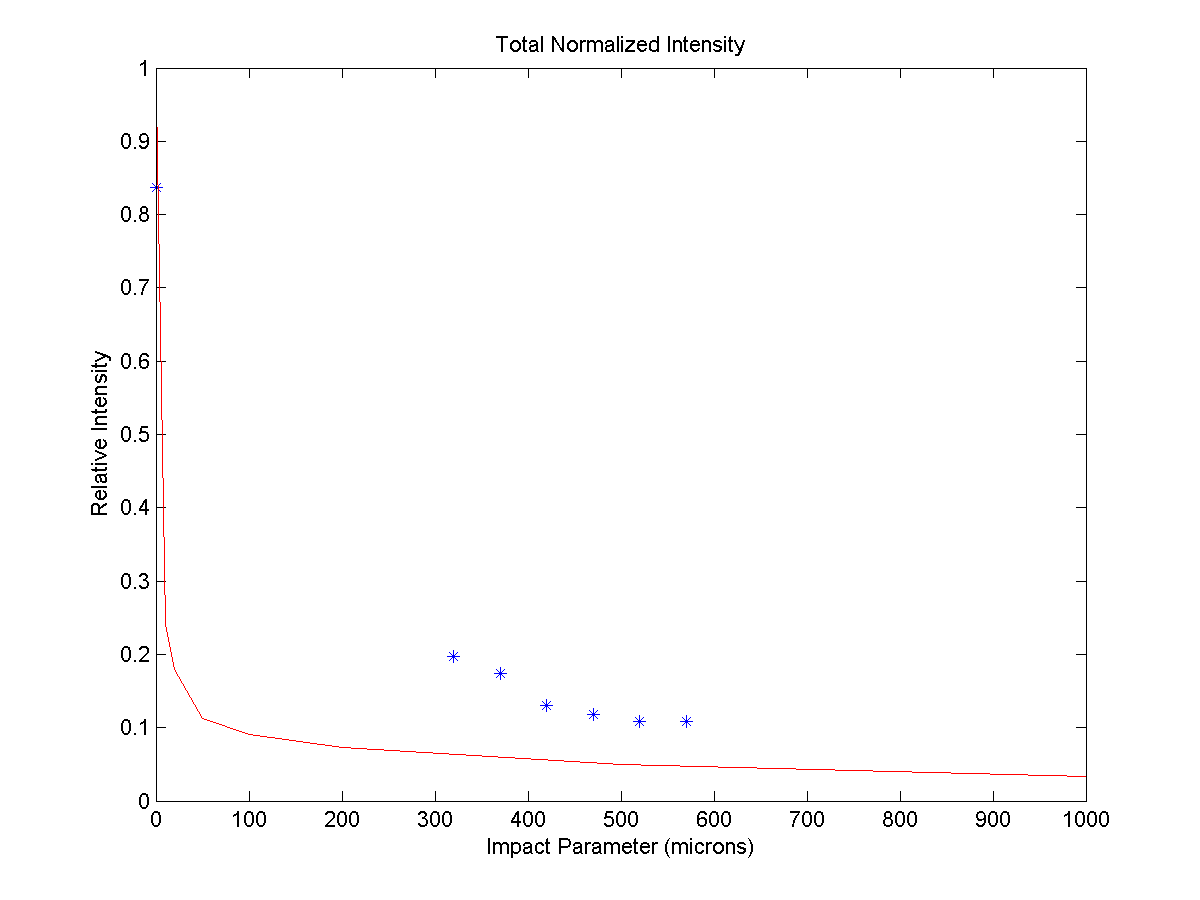
\includegraphics[scale=0.5]{Figures/Total_Intensity.PNG}
\caption{}
\end{center}
\end{figure}

\begin{figure}
\begin{center}
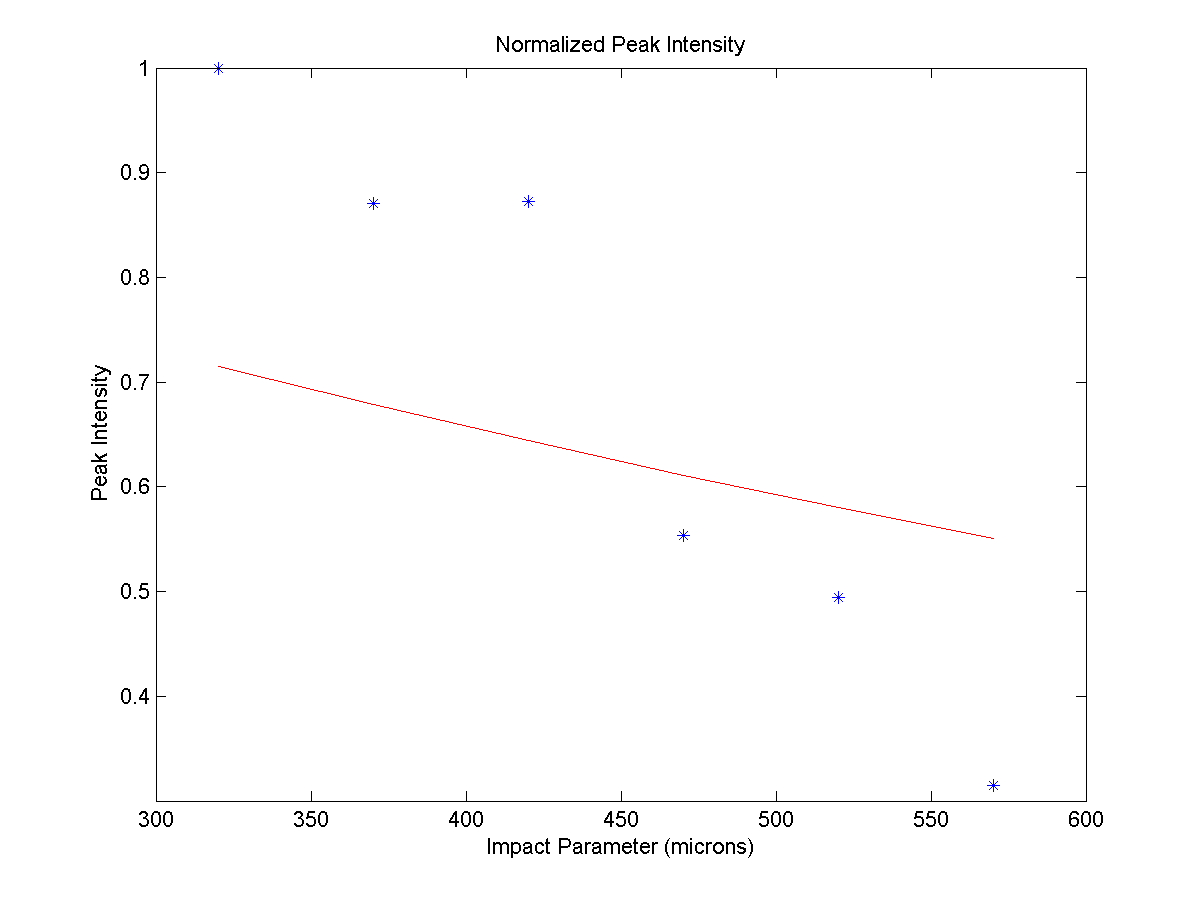
\includegraphics[scale=0.5]{Figures/PeakY_ODR.PNG}
\caption{}
\end{center}
\end{figure}

\begin{figure}
\begin{center}
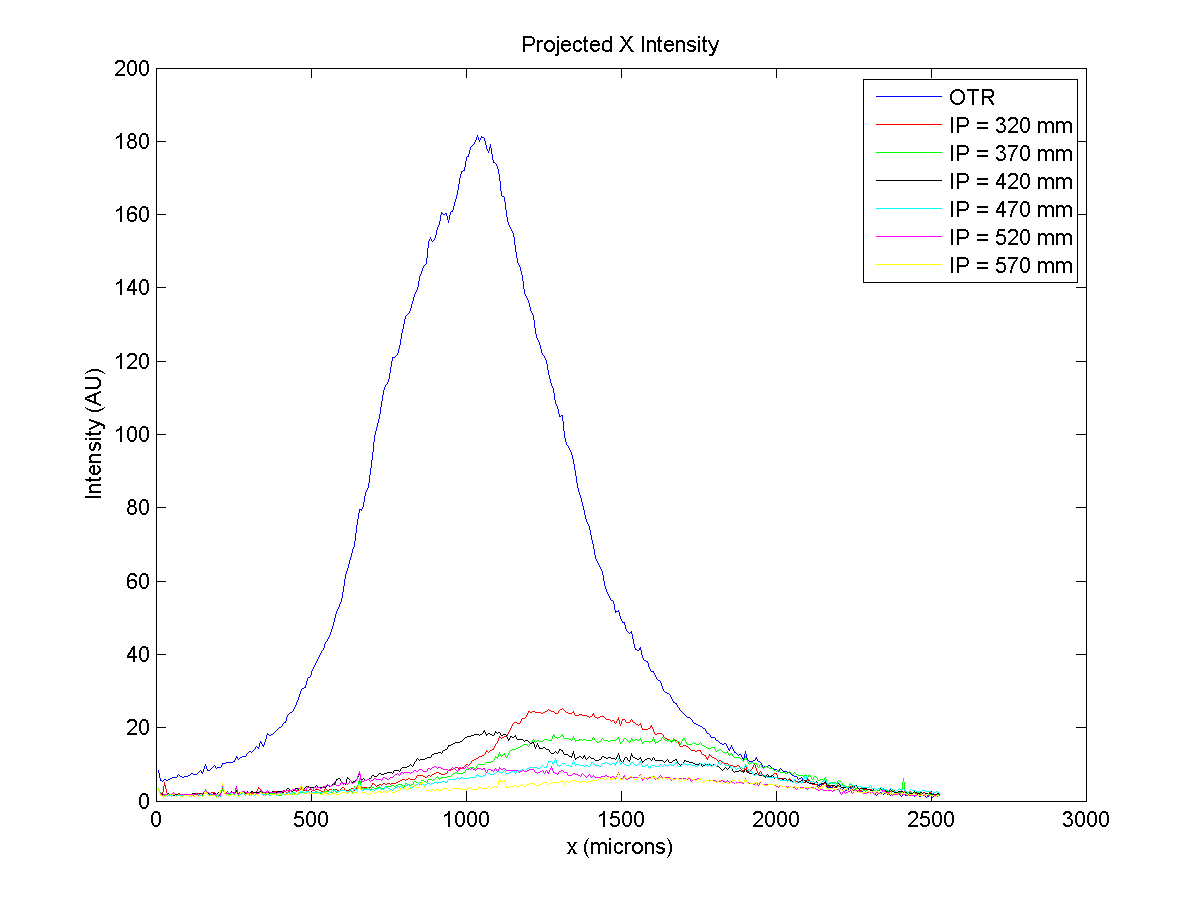
\includegraphics[scale=0.5]{Figures/XProj_ODR.PNG}
\caption{}
\end{center}
\end{figure}

\begin{figure}
\begin{center}
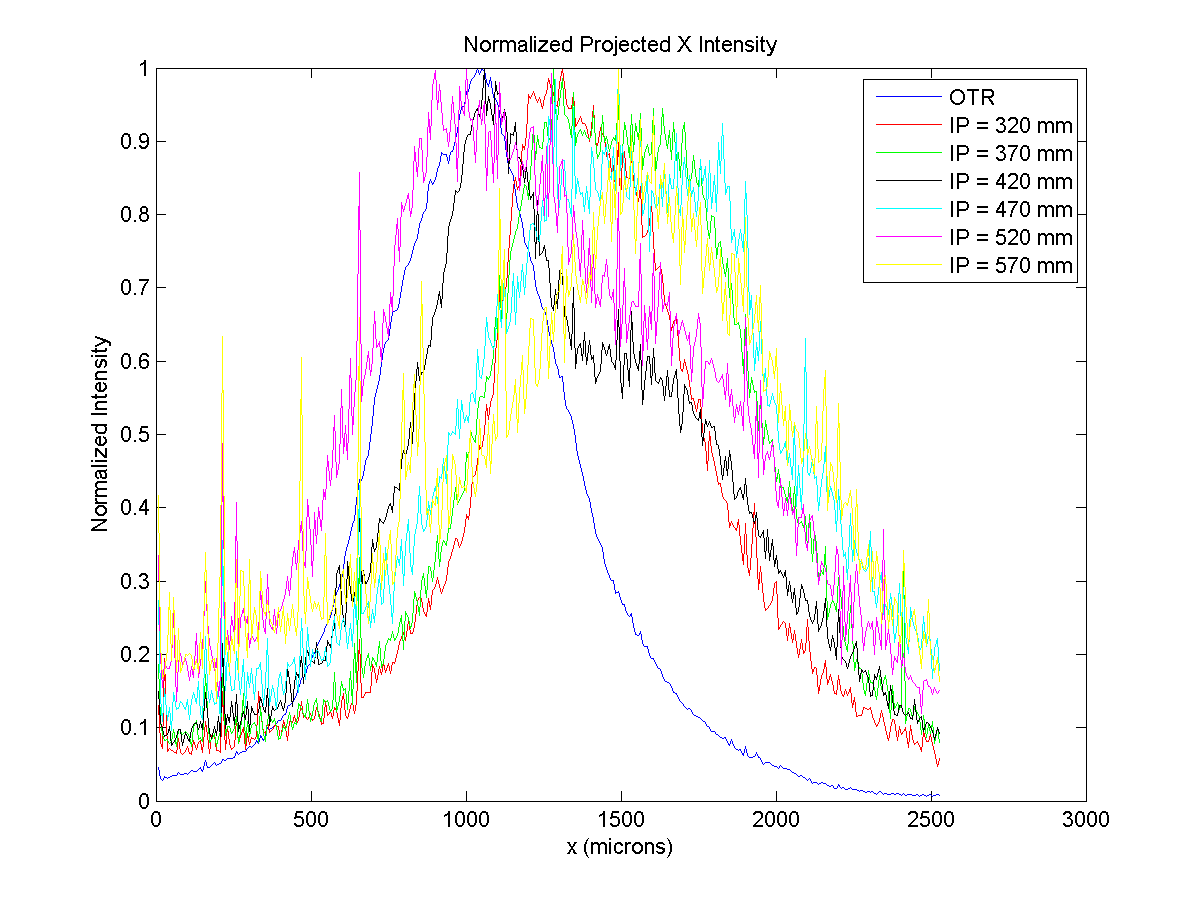
\includegraphics[scale=0.5]{Figures/XProj_Norm_ODR.PNG}
\caption{}
\end{center}
\end{figure}


\newpage

\section{Total Intensity}

These figures show the total intensity for ODR and OTR for each shot for 500 shots total.

\begin{figure}
\begin{center}
\includegraphics[scale=0.5]{Figures/PixelSum_ODR_0.PNG}
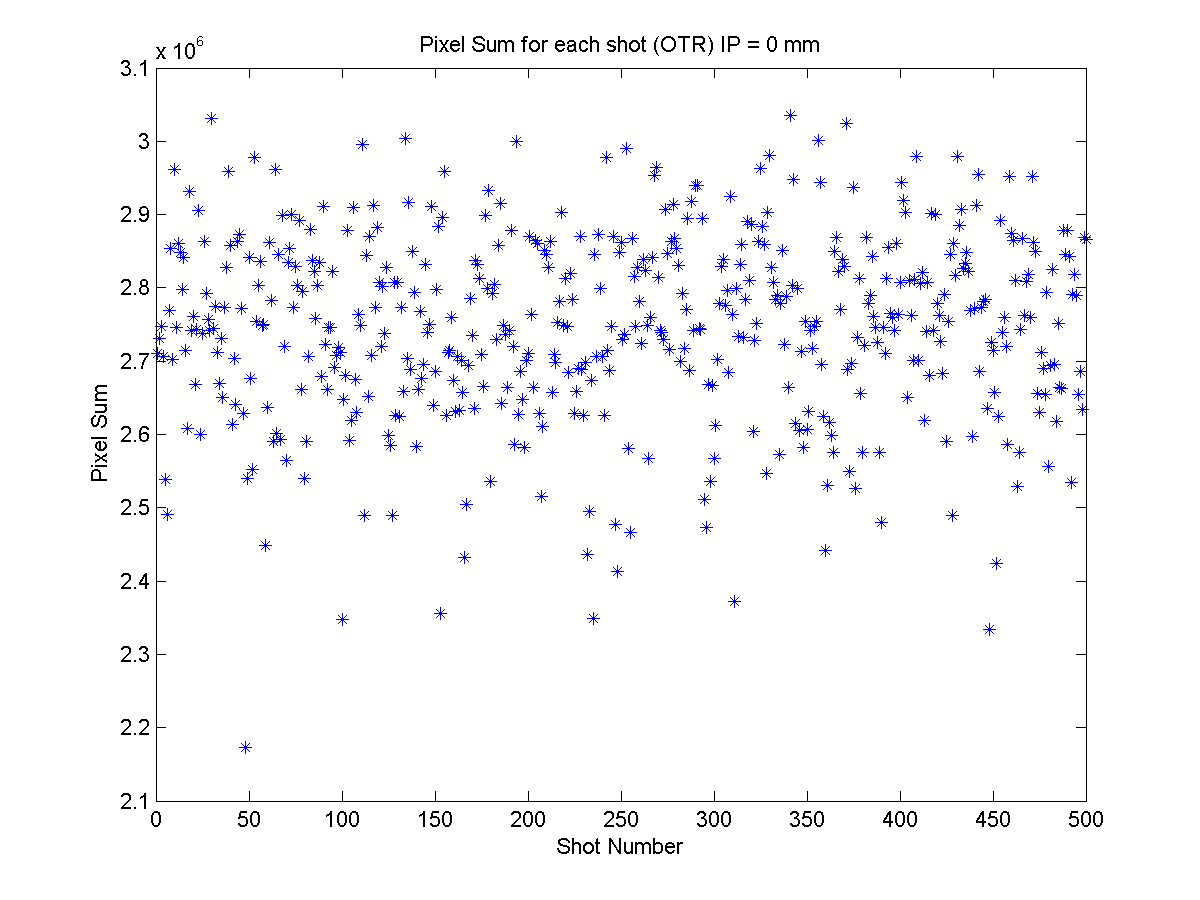
\includegraphics[scale=0.5]{Figures/PixelSum_OTR_0.PNG}
\caption{}
\end{center}
\end{figure}

\begin{figure}
\begin{center}
\includegraphics[scale=0.5]{Figures/PixelSum_ODR_320.PNG}
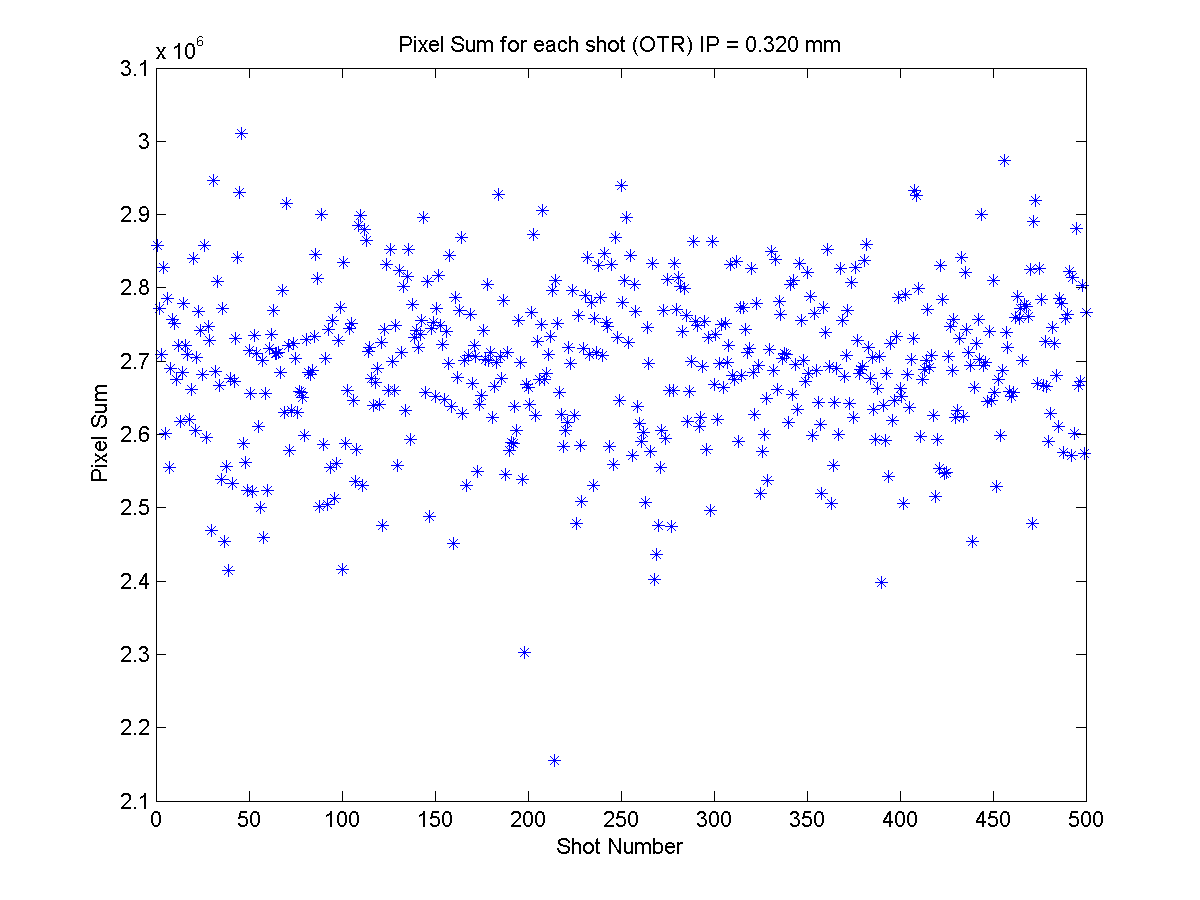
\includegraphics[scale=0.5]{Figures/PixelSum_OTR_320.PNG}
\caption{}
\end{center}
\end{figure}

\begin{figure}
\begin{center}
\includegraphics[scale=0.5]{Figures/PixelSum_ODR_370.PNG}
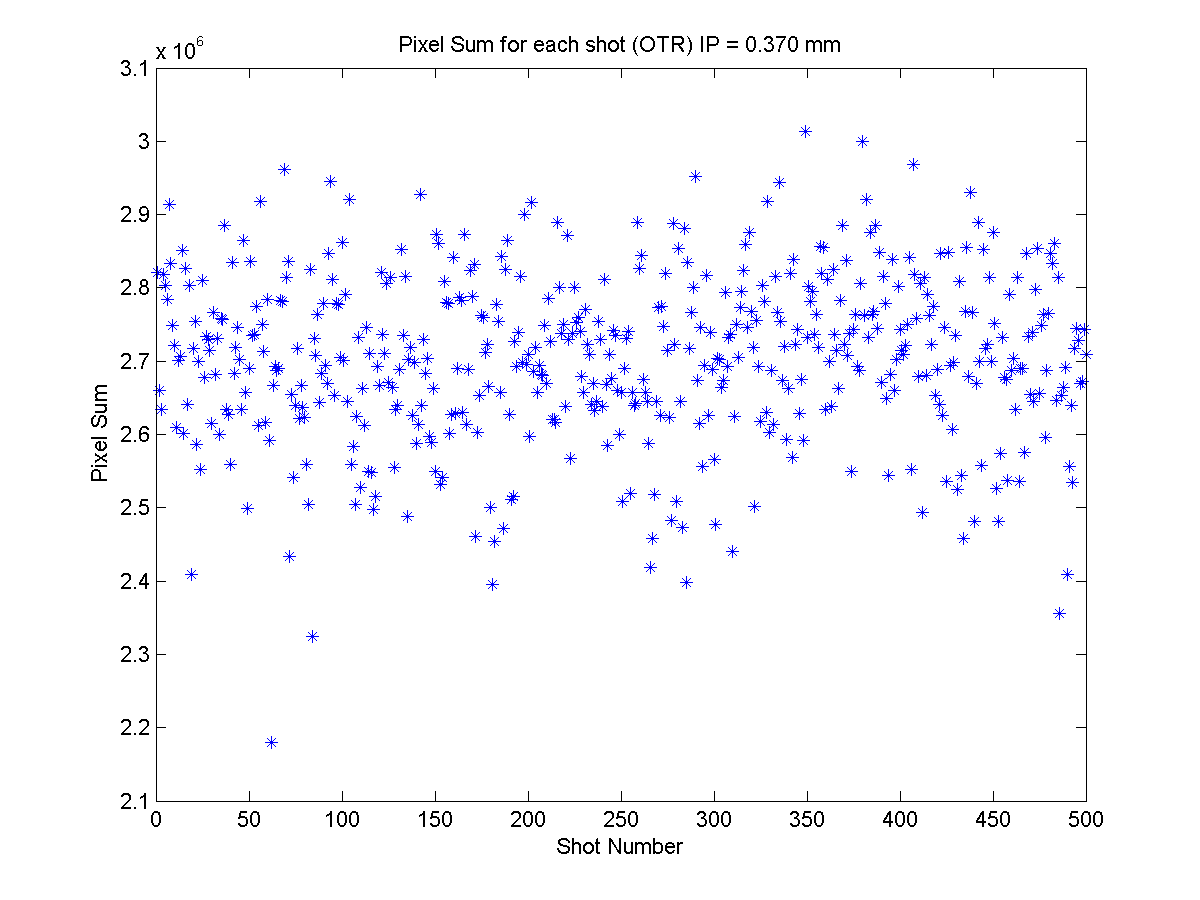
\includegraphics[scale=0.5]{Figures/PixelSum_OTR_370.PNG}
\caption{}
\end{center}
\end{figure}

\begin{figure}
\begin{center}
\includegraphics[scale=0.5]{Figures/PixelSum_ODR_420.PNG}
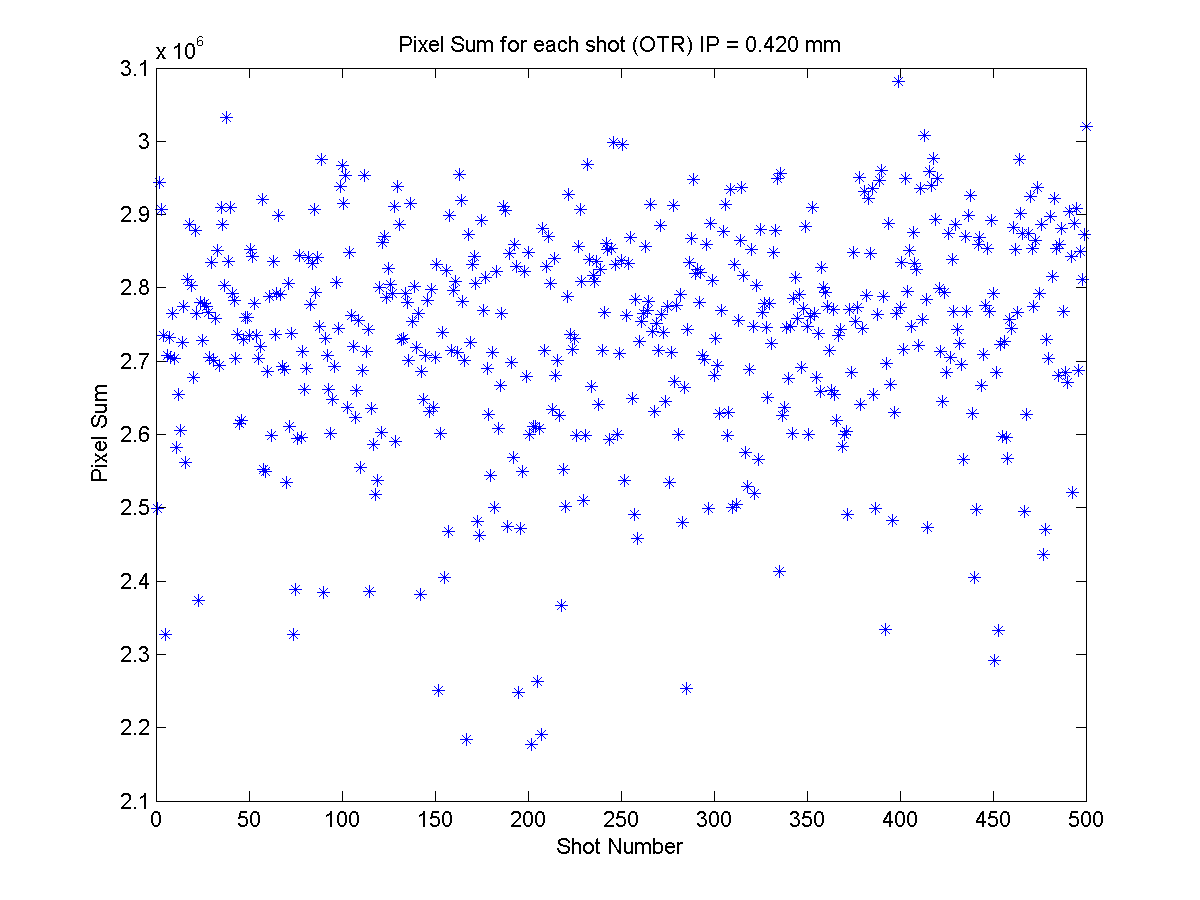
\includegraphics[scale=0.5]{Figures/PixelSum_OTR_420.PNG}
\caption{}
\end{center}
\end{figure}

\begin{figure}
\begin{center}
\includegraphics[scale=0.5]{Figures/PixelSum_ODR_470.PNG}
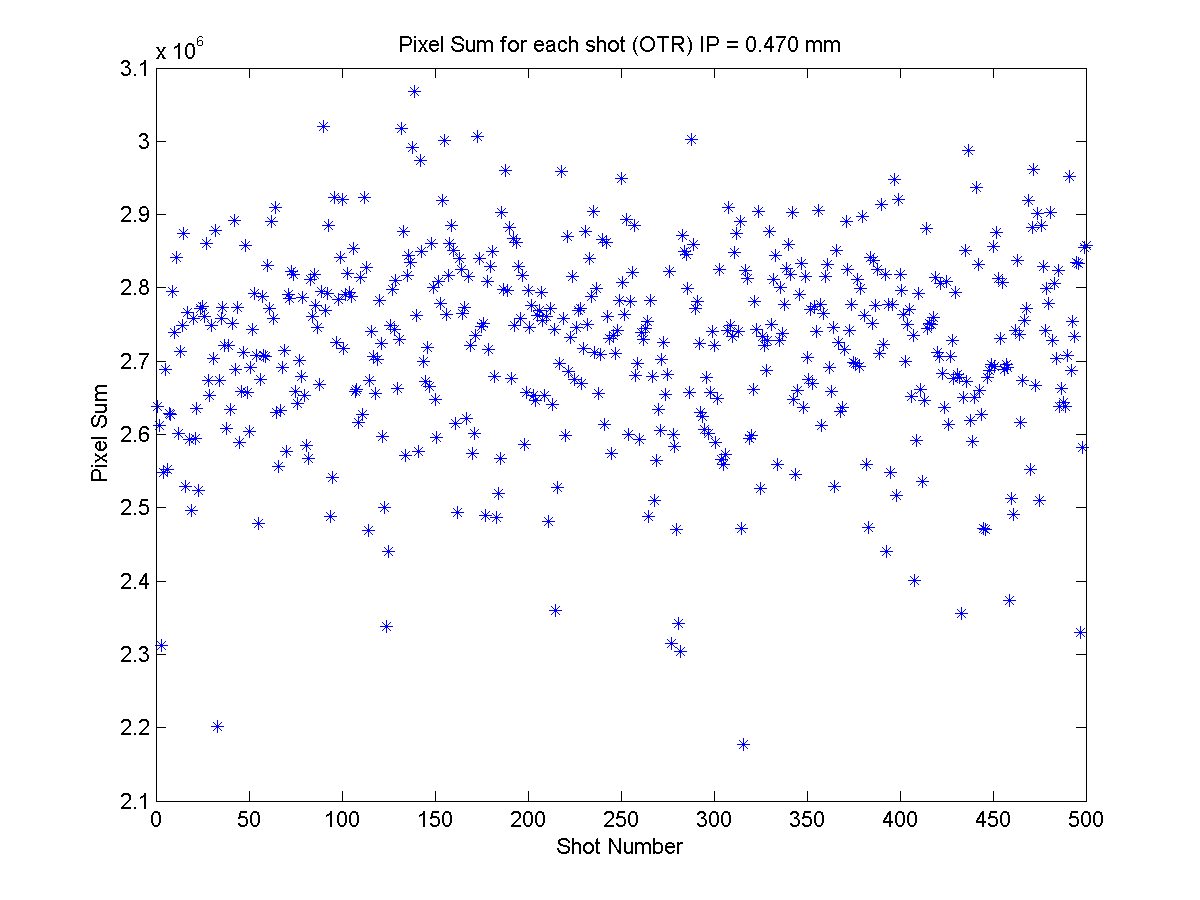
\includegraphics[scale=0.5]{Figures/PixelSum_OTR_470.PNG}
\caption{}
\end{center}
\end{figure}

\begin{figure}
\begin{center}
\includegraphics[scale=0.5]{Figures/PixelSum_ODR_520.PNG}
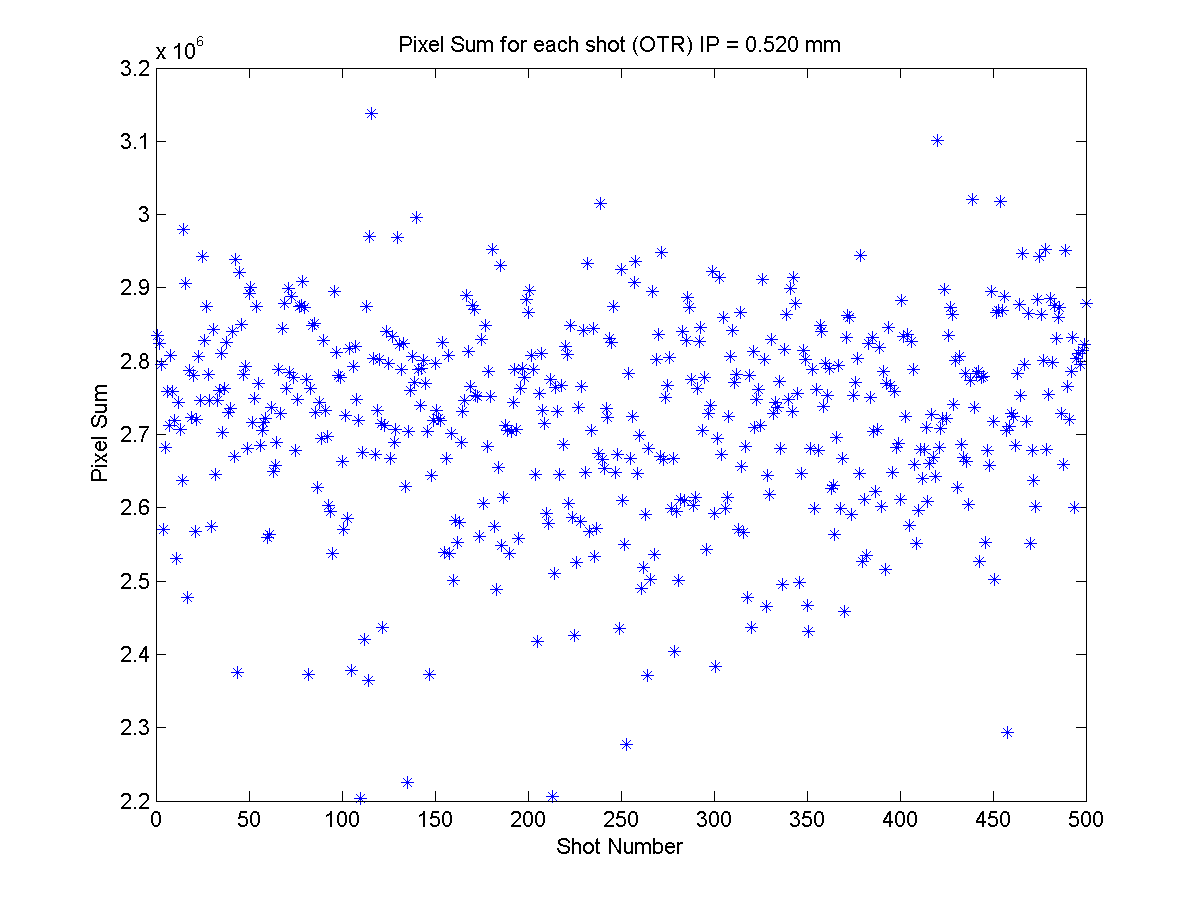
\includegraphics[scale=0.5]{Figures/PixelSum_OTR_520.PNG}
\caption{}
\end{center}
\end{figure}

\begin{figure}
\begin{center}
\includegraphics[scale=0.5]{Figures/PixelSum_ODR_570.PNG}
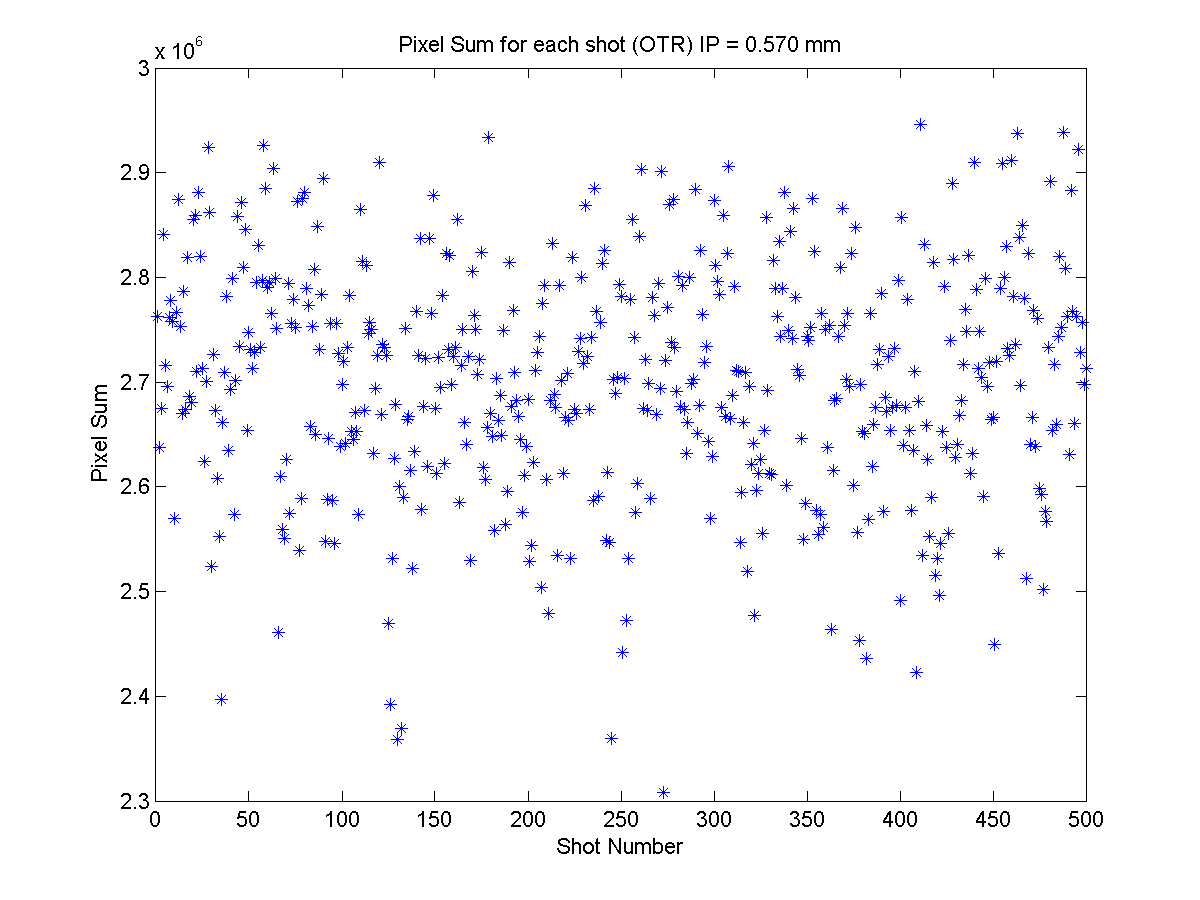
\includegraphics[scale=0.5]{Figures/PixelSum_OTR_570.PNG}
\caption{}
\end{center}
\end{figure}



newpage

\section{Projected X Intensity}

These figures show the projected X intensity for ODR and OTR for each shot for 500 shots total.

\begin{figure}
\begin{center}
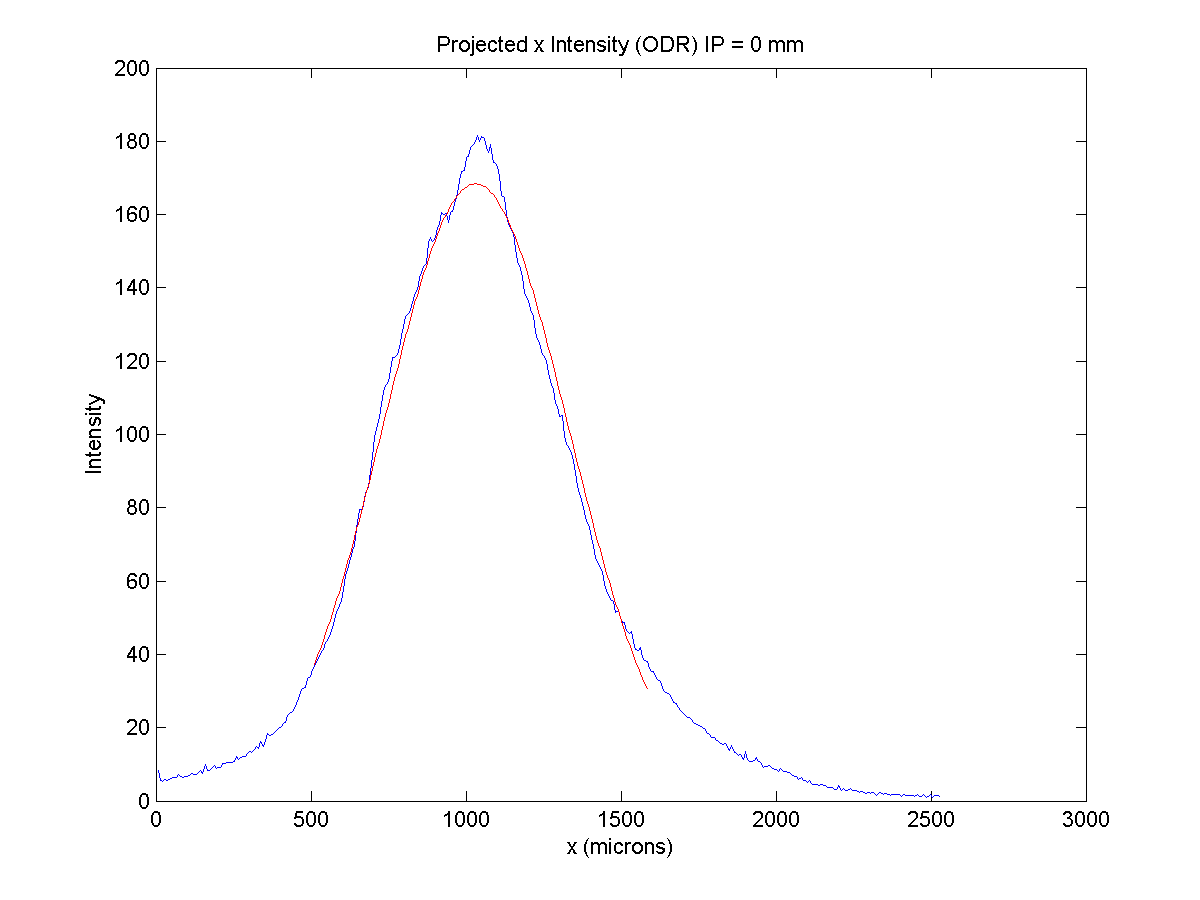
\includegraphics[scale=0.5]{Figures/ProjX_ODR_0.PNG}
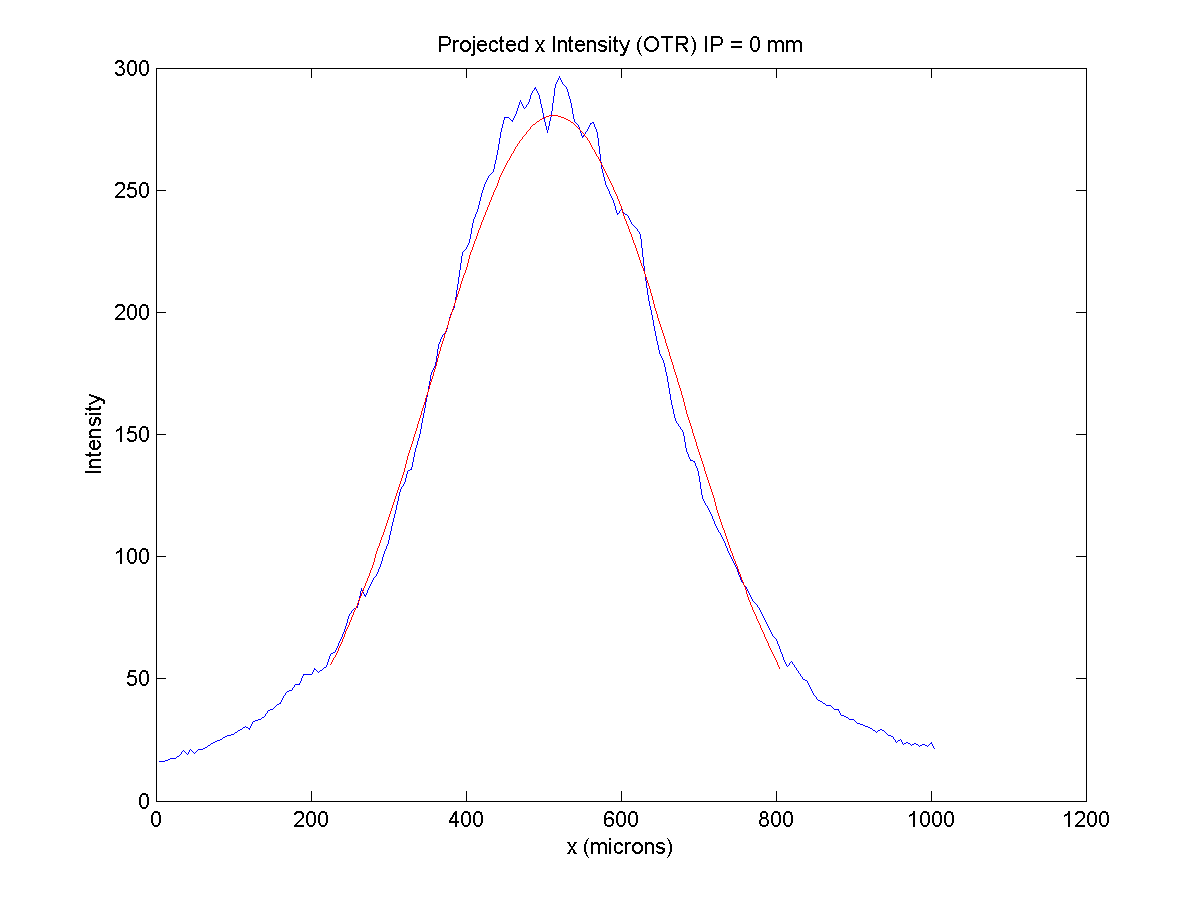
\includegraphics[scale=0.5]{Figures/ProjX_OTR_0.PNG}
\caption{}
\end{center}
\end{figure}

\begin{figure}
\begin{center}
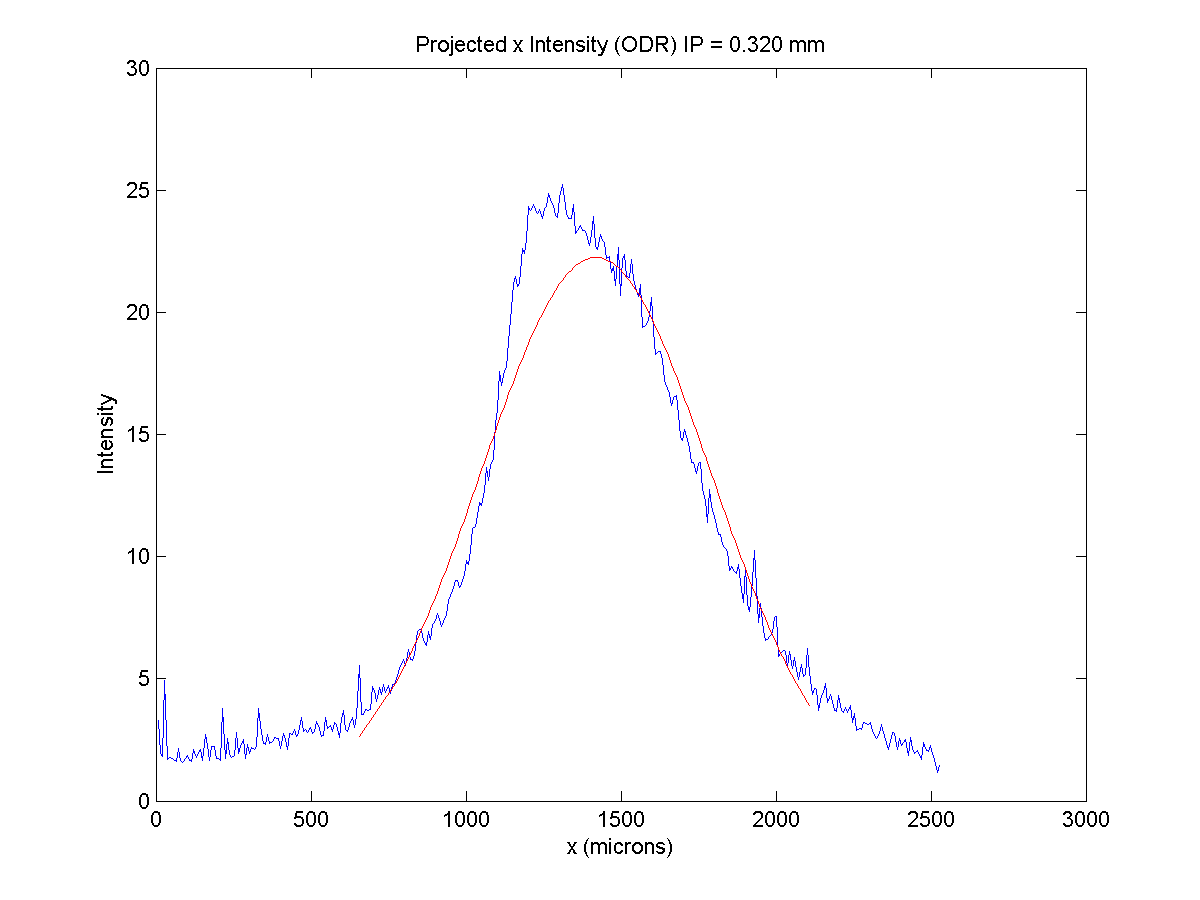
\includegraphics[scale=0.5]{Figures/ProjX_ODR_320.PNG}
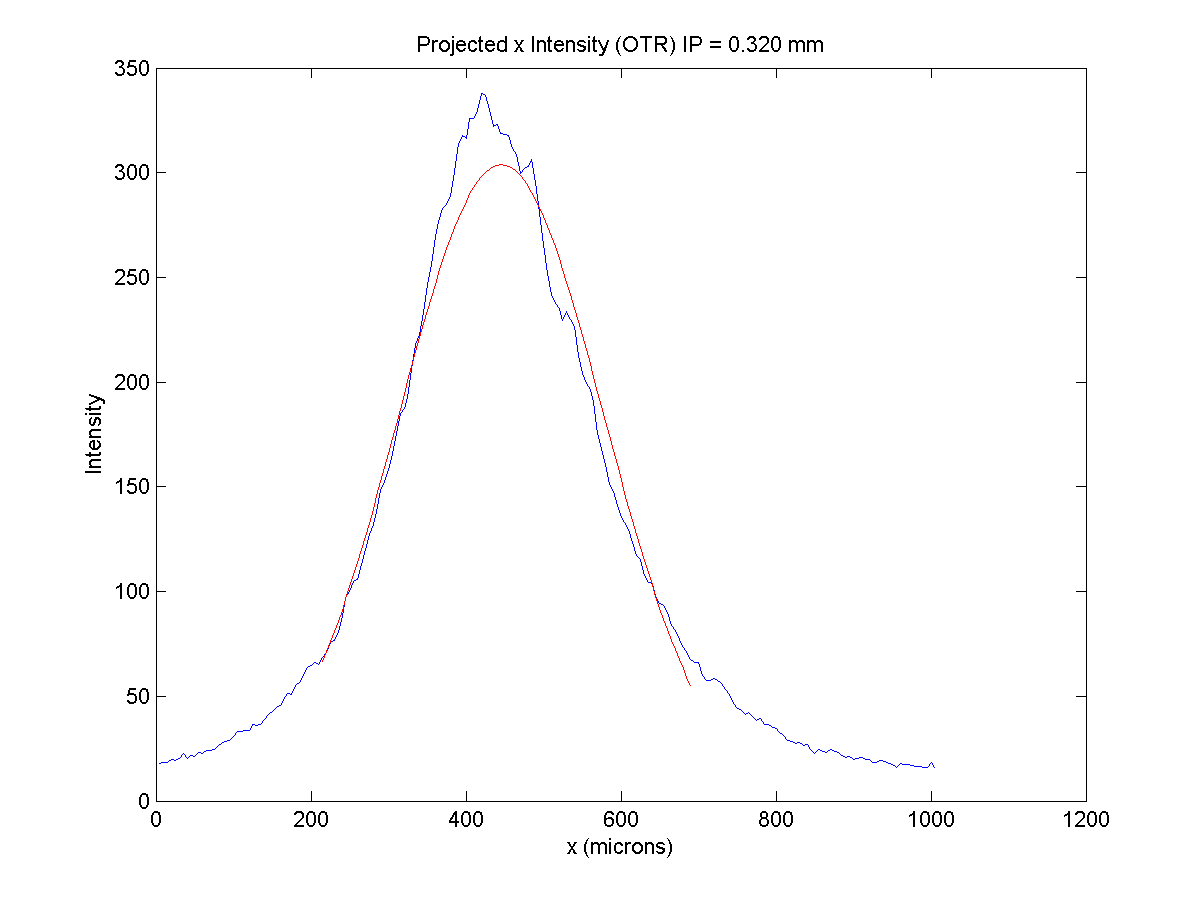
\includegraphics[scale=0.5]{Figures/ProjX_OTR_320.PNG}
\caption{}
\end{center}
\end{figure}

\begin{figure}
\begin{center}
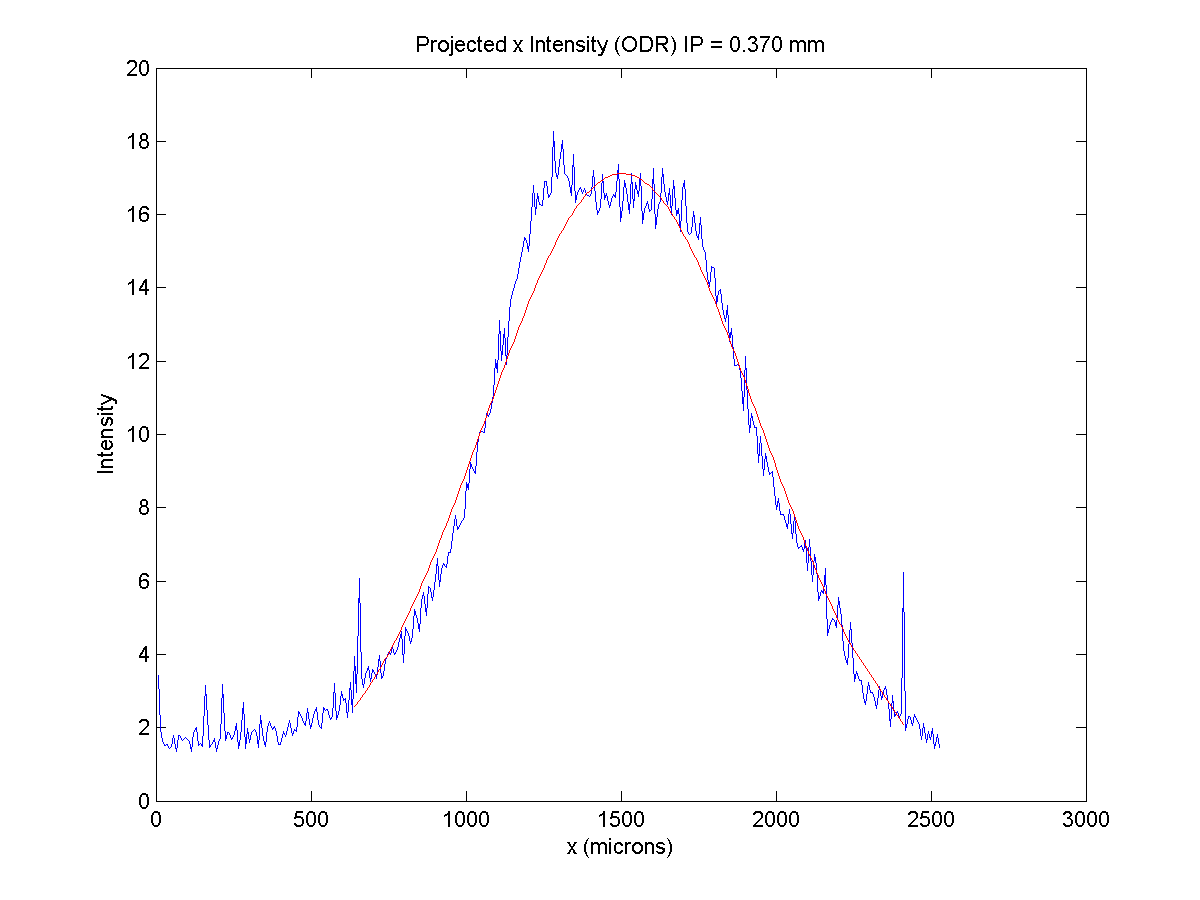
\includegraphics[scale=0.5]{Figures/ProjX_ODR_370.PNG}
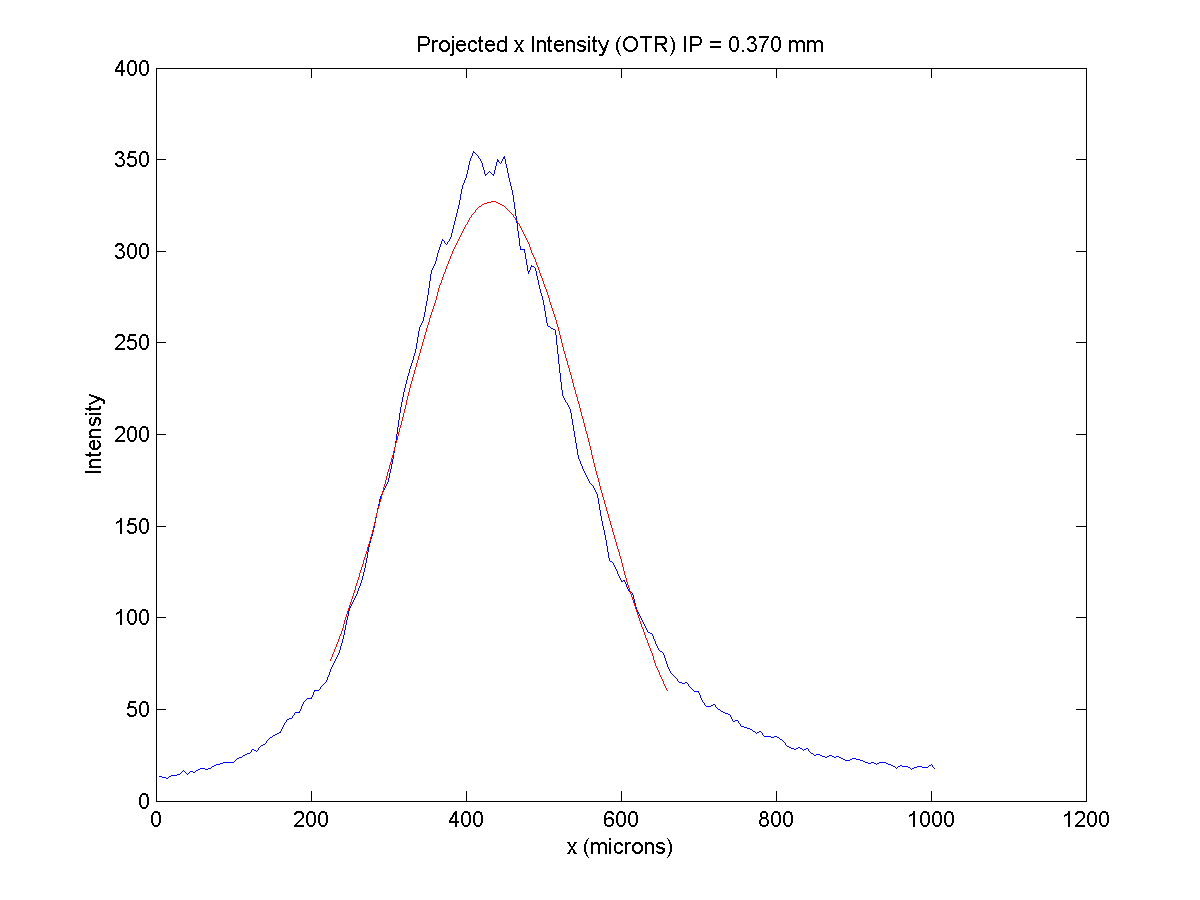
\includegraphics[scale=0.5]{Figures/ProjX_OTR_370.PNG}
\caption{}
\end{center}
\end{figure}

\begin{figure}
\begin{center}
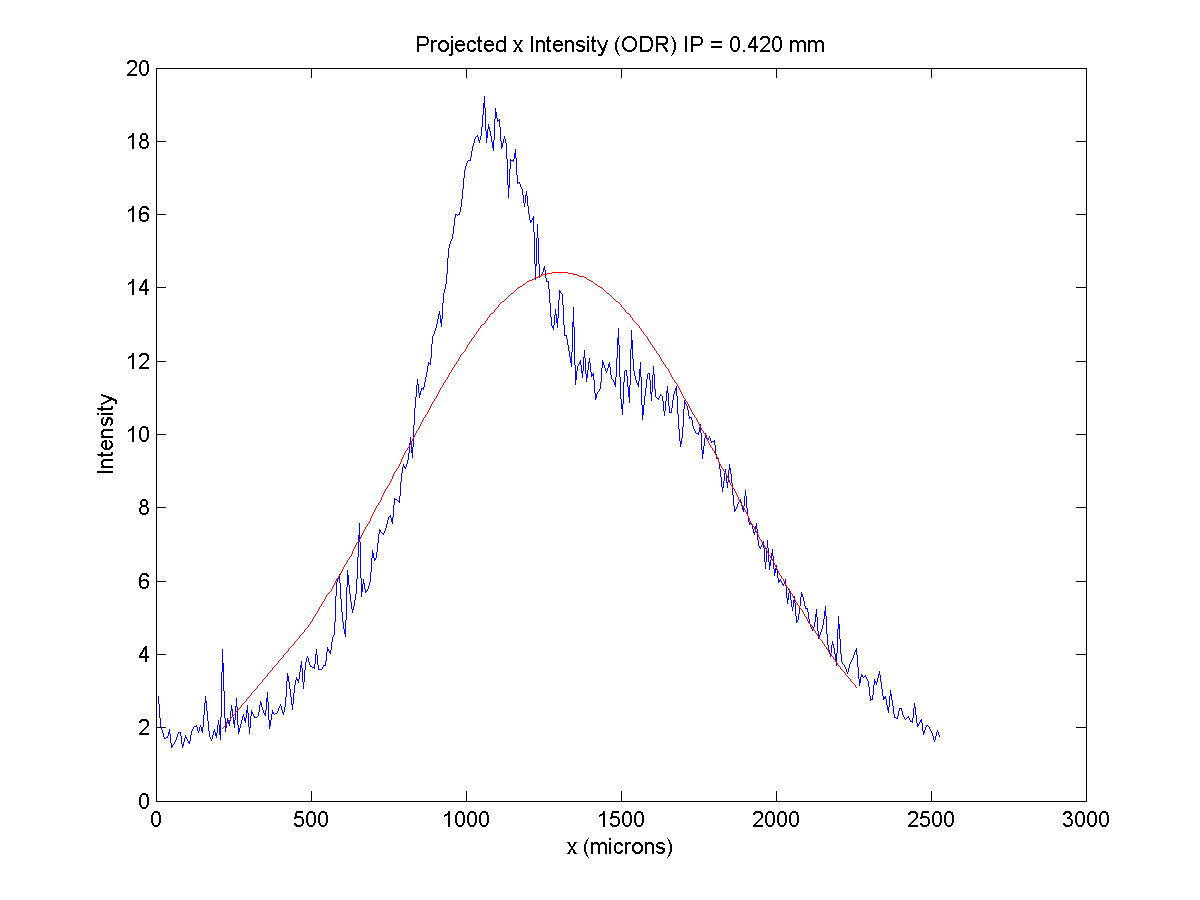
\includegraphics[scale=0.5]{Figures/ProjX_ODR_420.PNG}
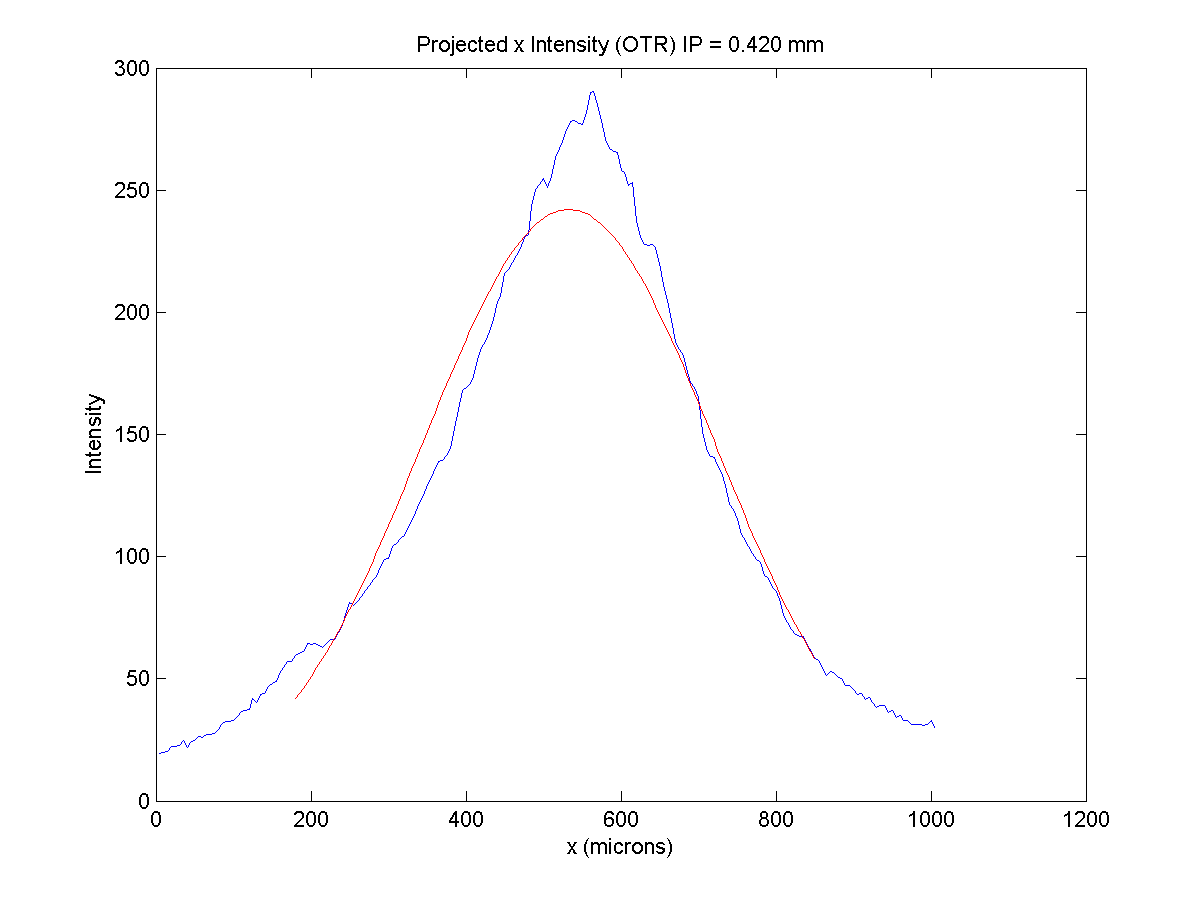
\includegraphics[scale=0.5]{Figures/ProjX_OTR_420.PNG}
\caption{}
\end{center}
\end{figure}

\begin{figure}
\begin{center}
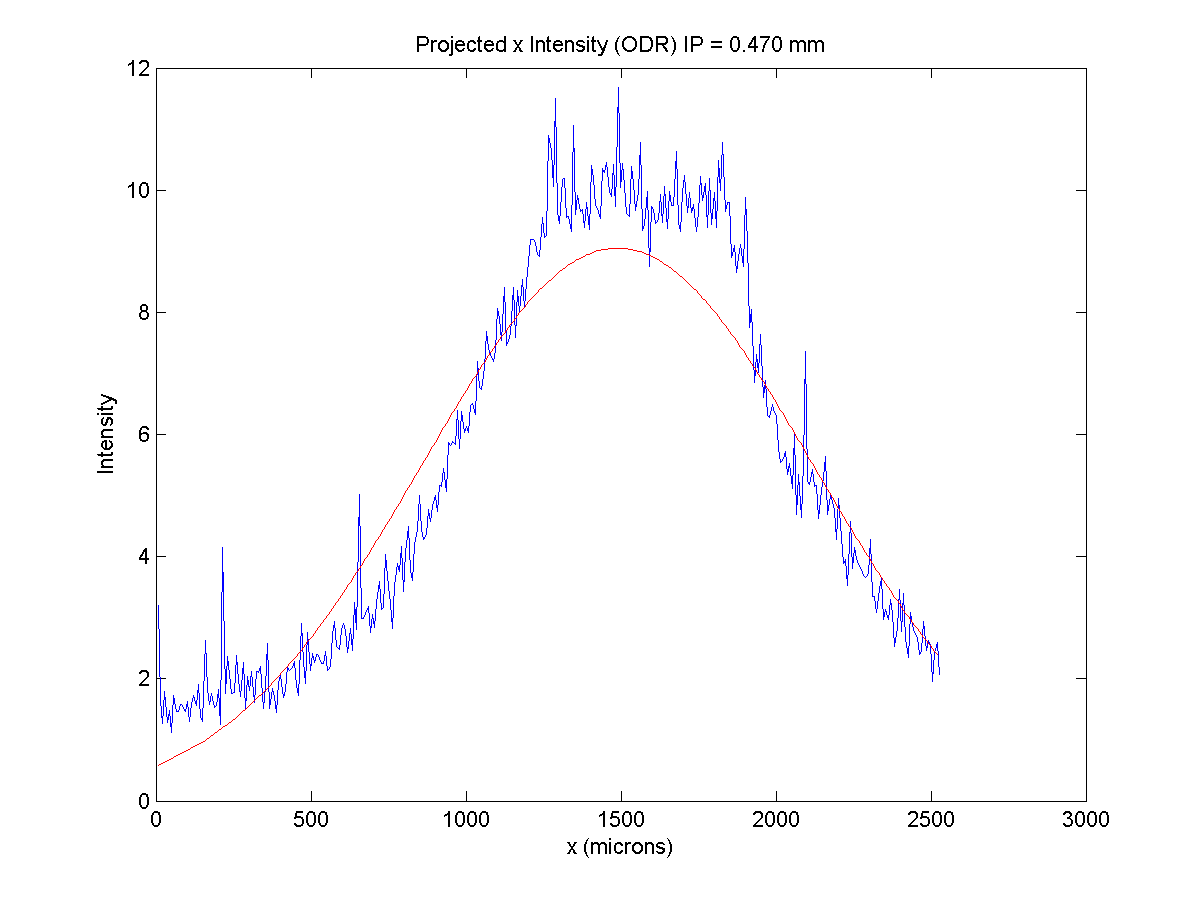
\includegraphics[scale=0.5]{Figures/ProjX_ODR_470.PNG}
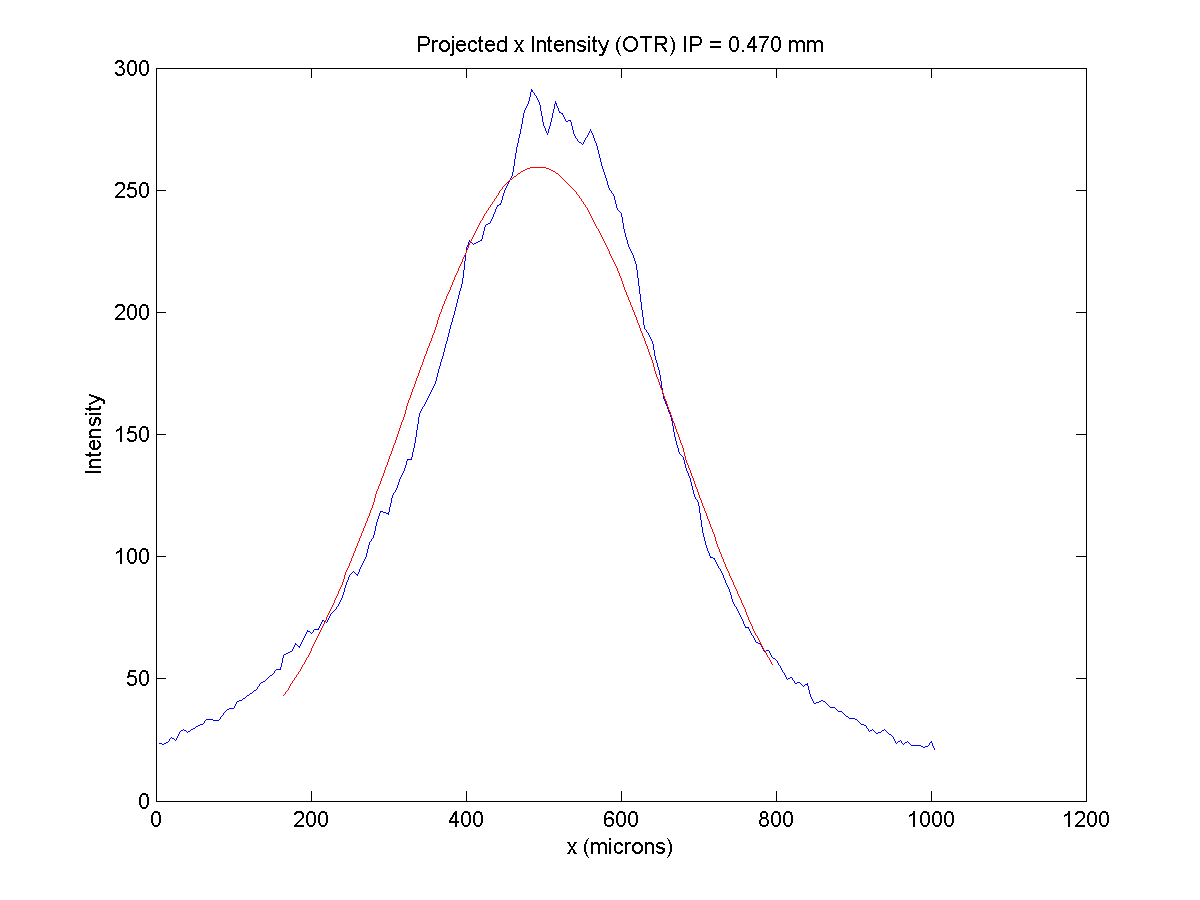
\includegraphics[scale=0.5]{Figures/ProjX_OTR_470.PNG}
\caption{}
\end{center}
\end{figure}

\begin{figure}
\begin{center}
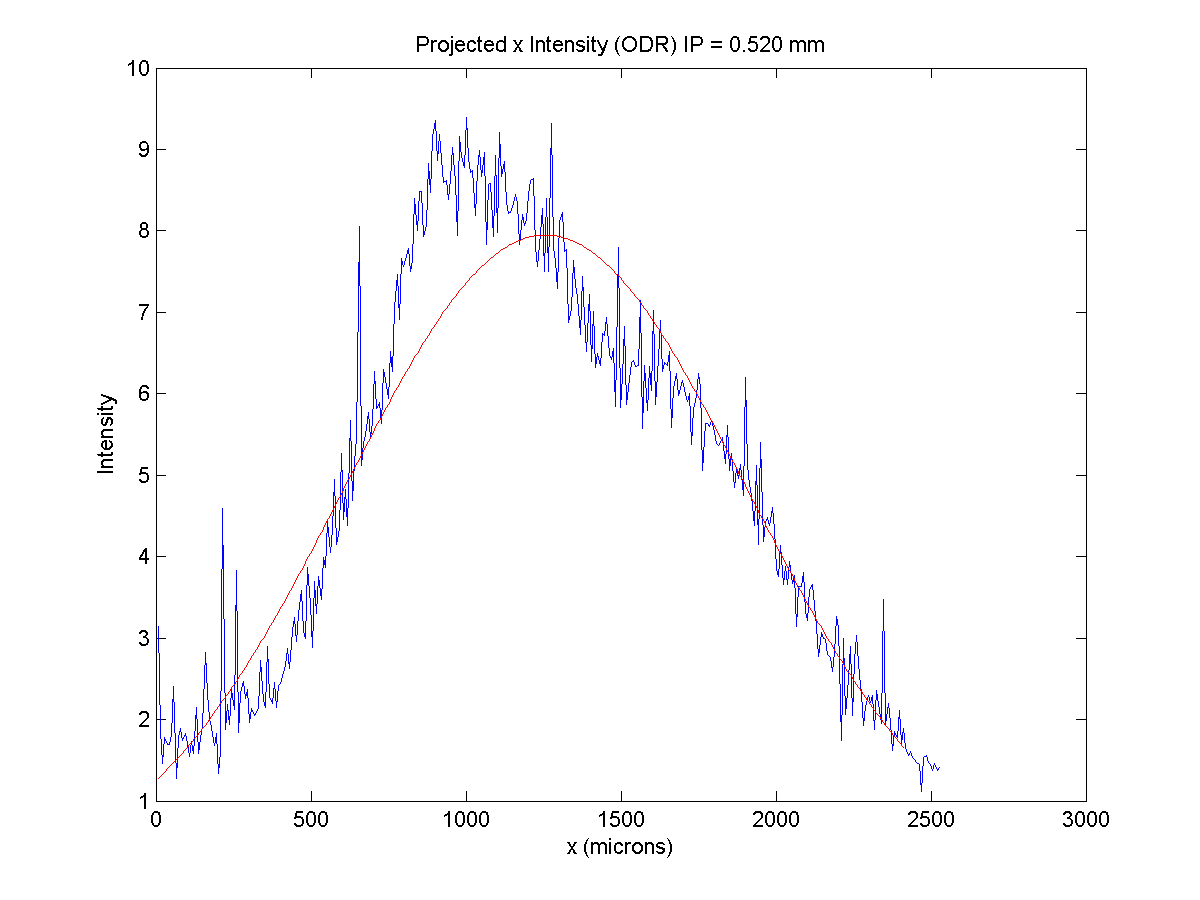
\includegraphics[scale=0.5]{Figures/ProjX_ODR_520.PNG}
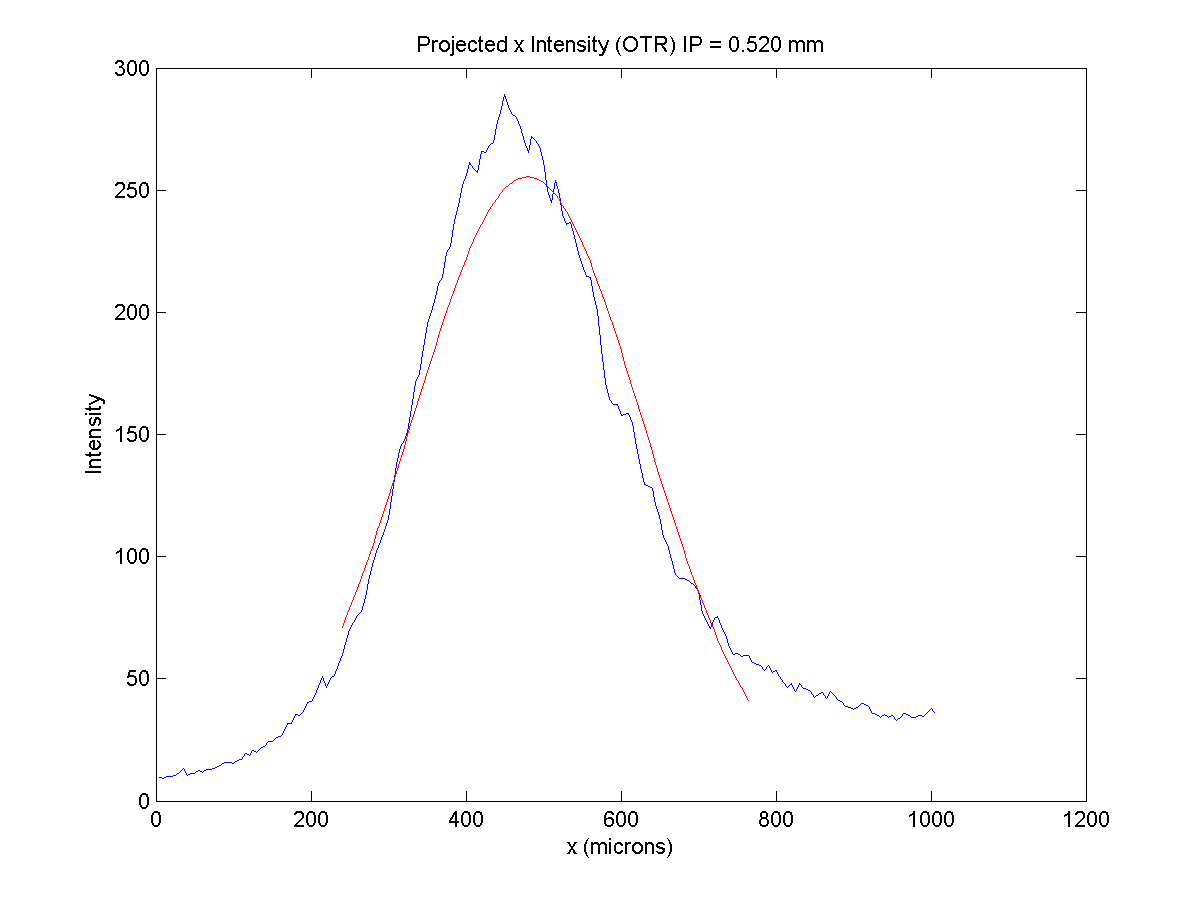
\includegraphics[scale=0.5]{Figures/ProjX_OTR_520.PNG}
\caption{}
\end{center}
\end{figure}

\begin{figure}
\begin{center}
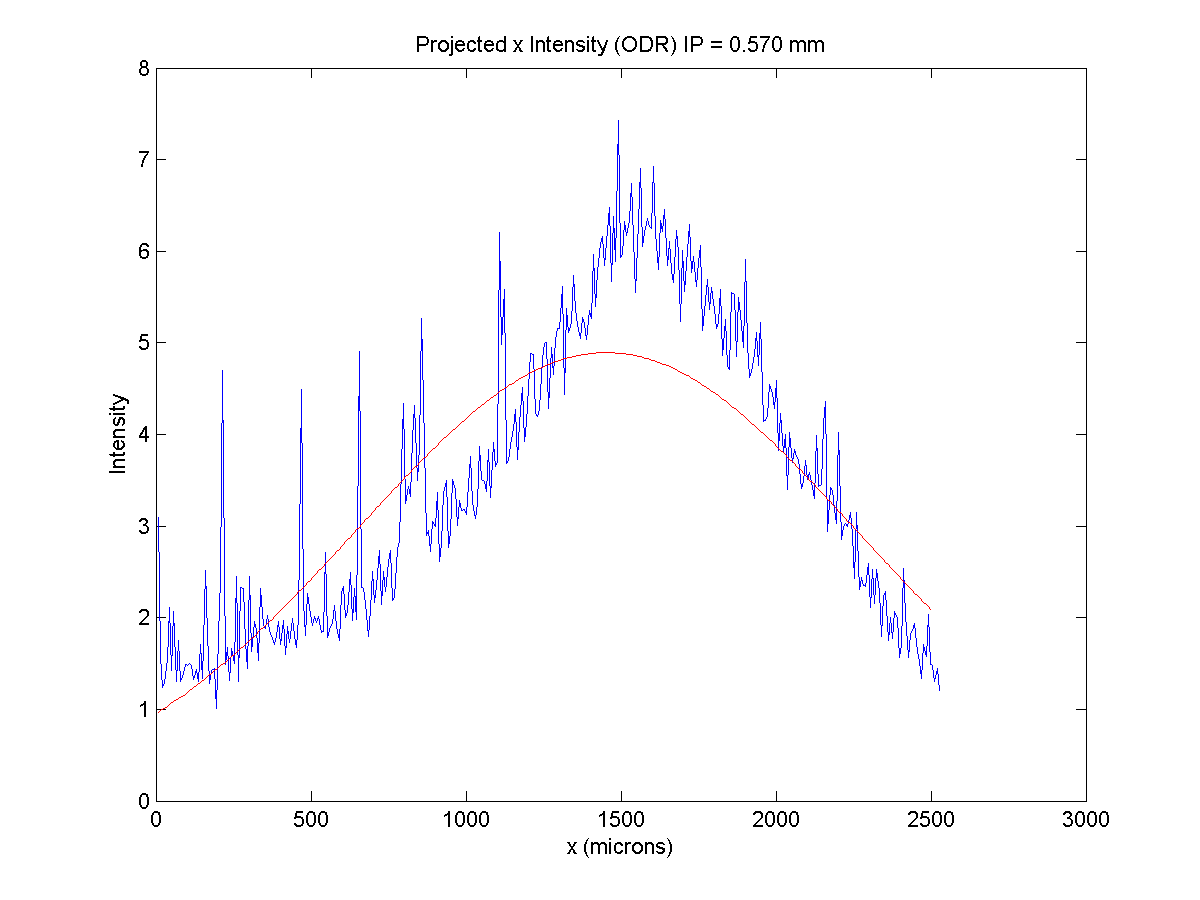
\includegraphics[scale=0.5]{Figures/ProjX_ODR_570.PNG}
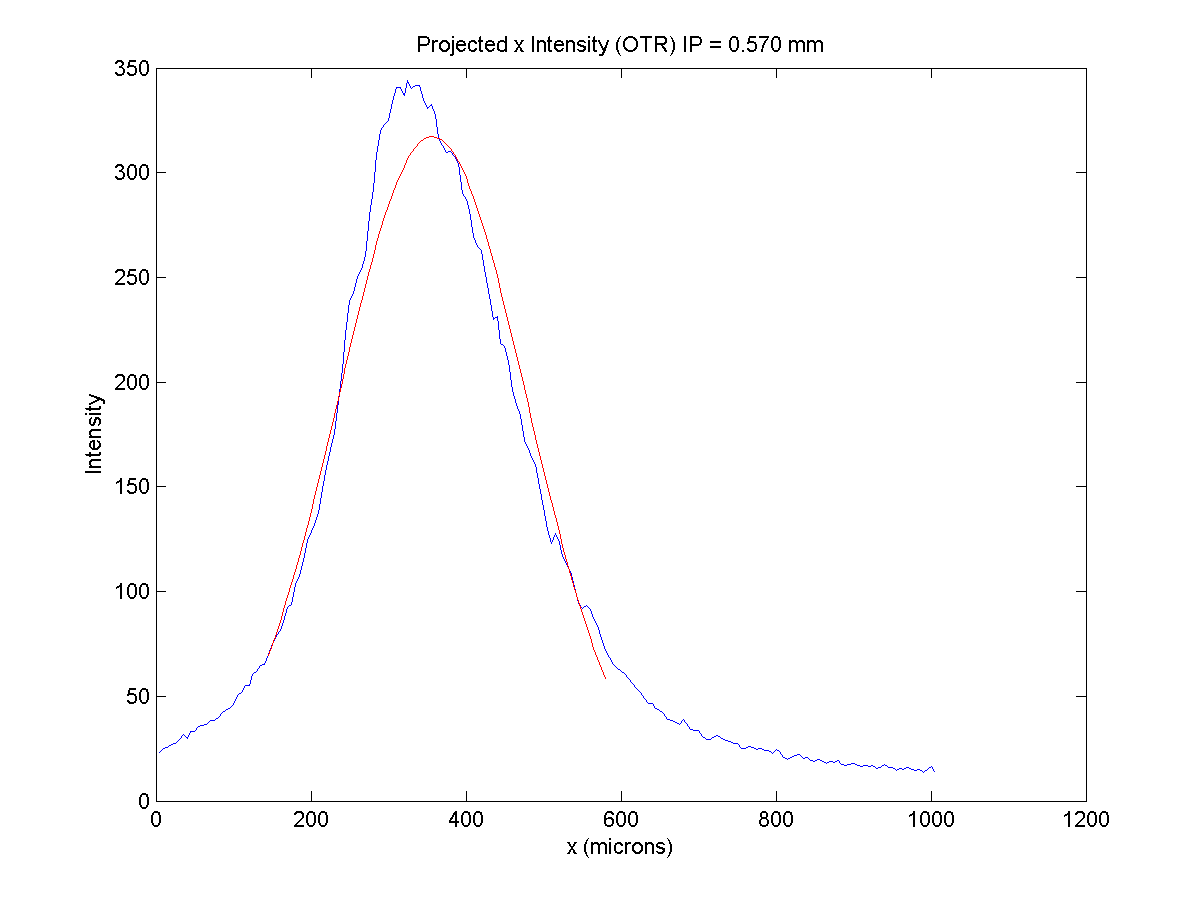
\includegraphics[scale=0.5]{Figures/ProjX_OTR_570.PNG}
\caption{}
\end{center}
\end{figure}



\newpage

\section{Projected Y Intensity}

These figures show the projected Y intensity for ODR and OTR for each shot for 500 shots total.

\begin{figure}
\begin{center}
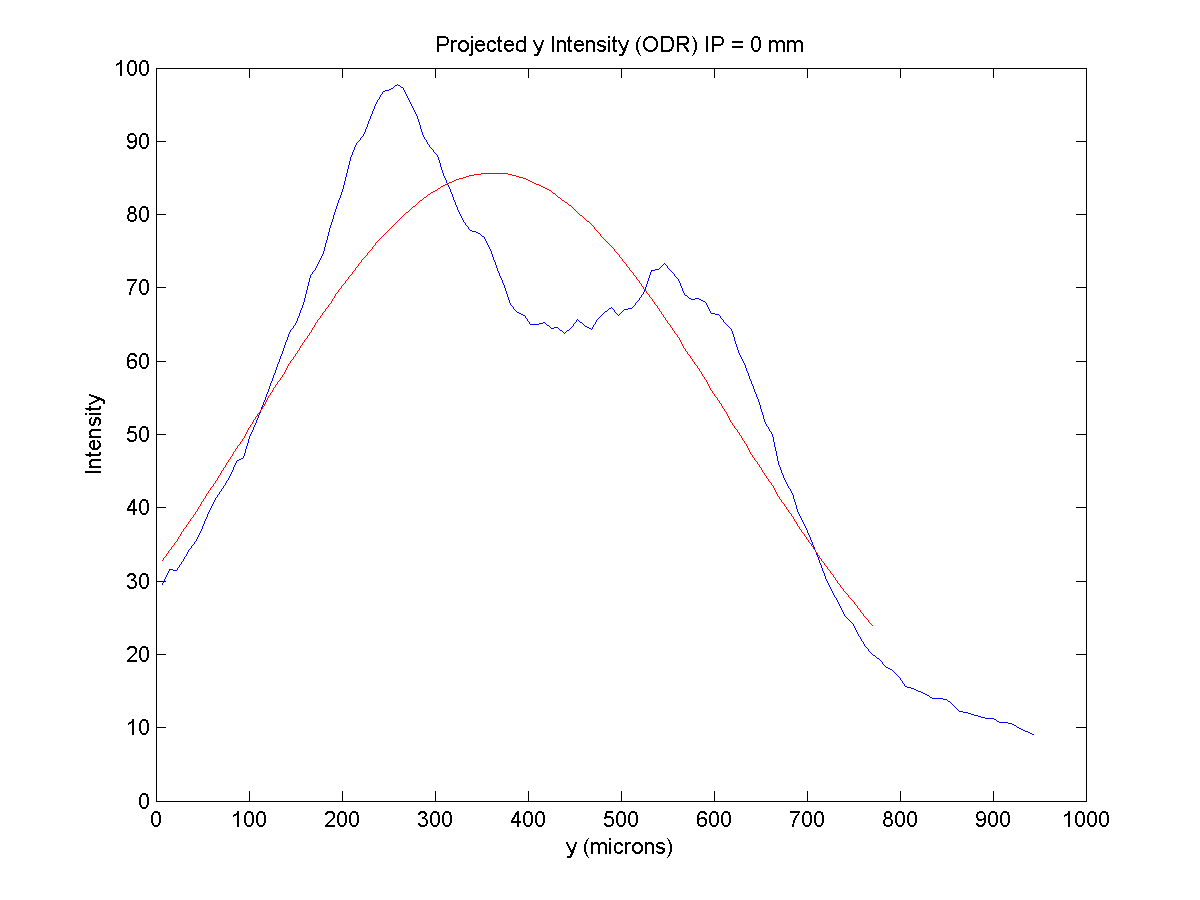
\includegraphics[scale=0.5]{Figures/ProjY_ODR_0.PNG}
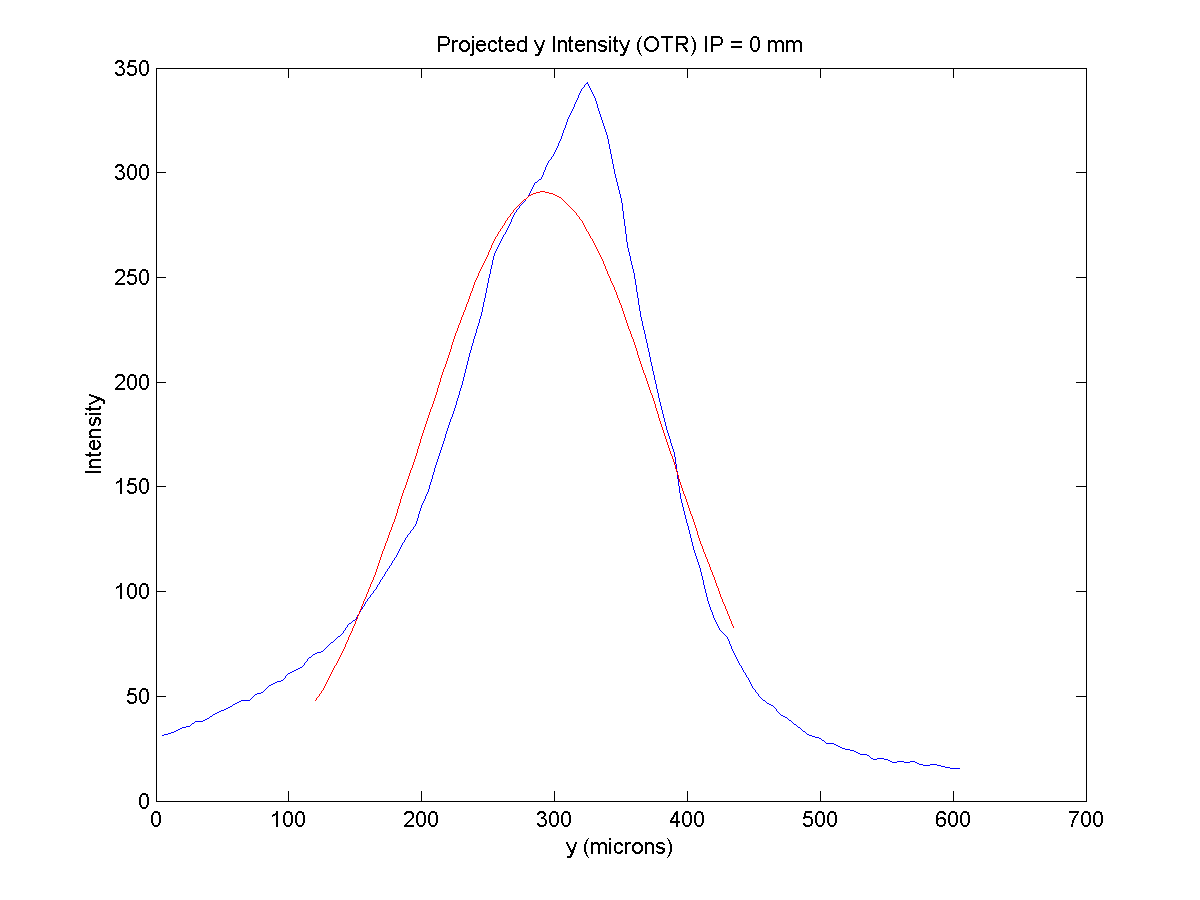
\includegraphics[scale=0.5]{Figures/ProjY_OTR_0.PNG}
\caption{}
\end{center}
\end{figure}

\begin{figure}
\begin{center}
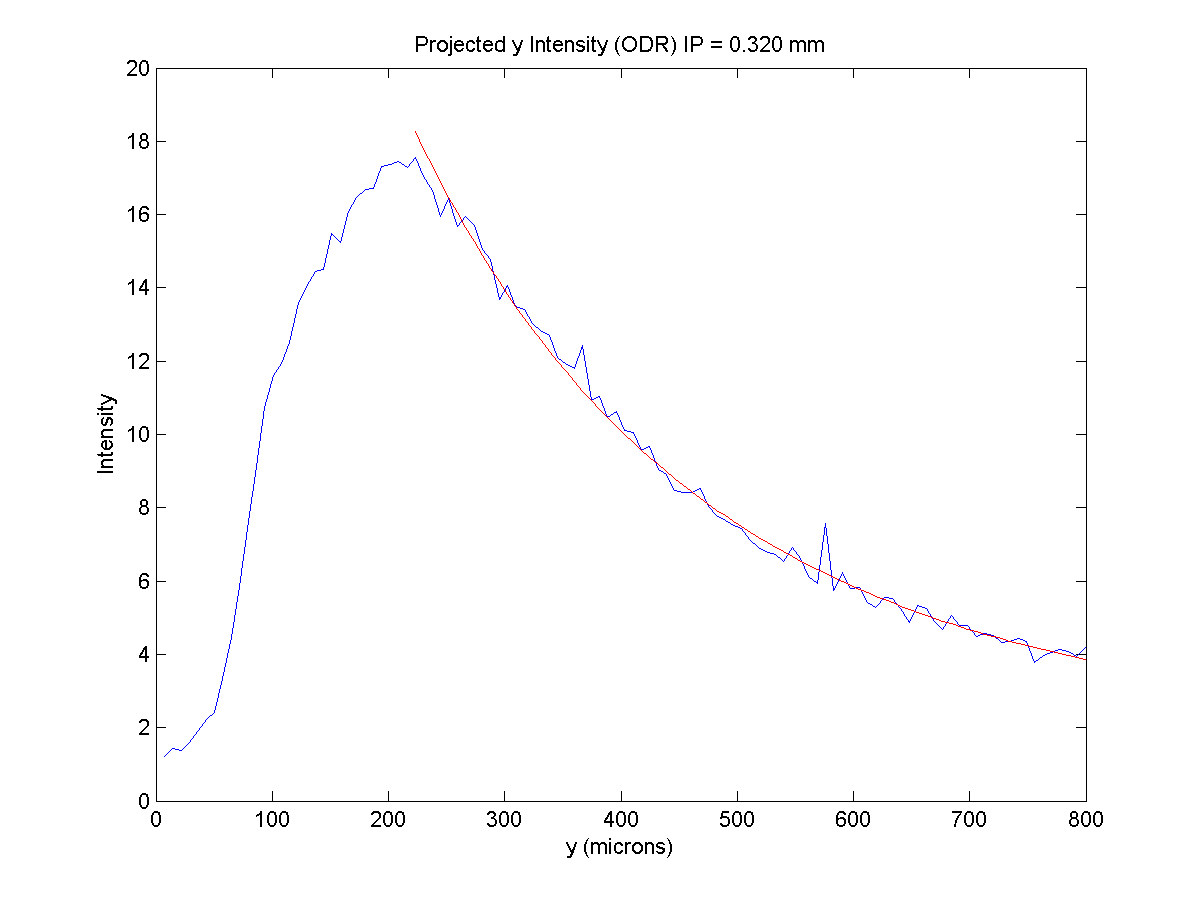
\includegraphics[scale=0.5]{Figures/ProjY_ODR_320.PNG}
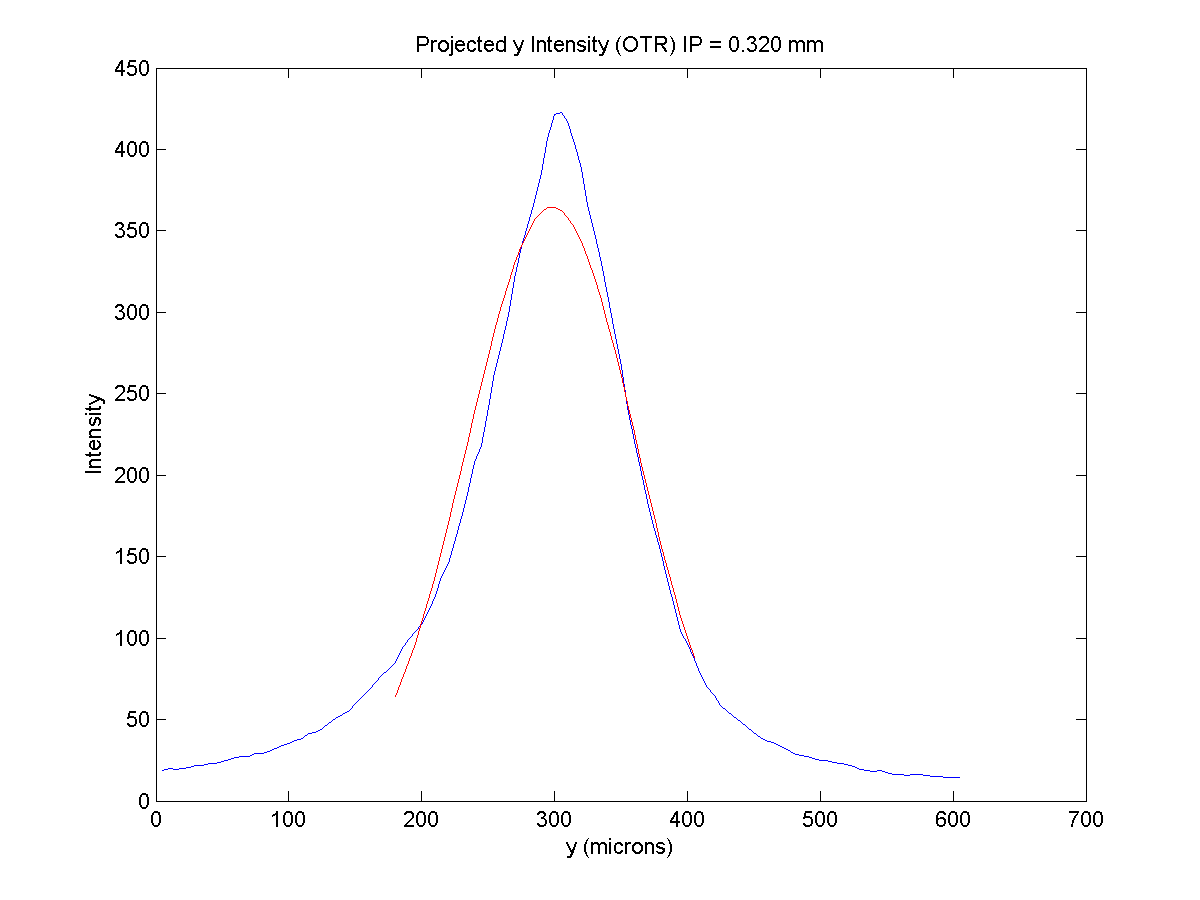
\includegraphics[scale=0.5]{Figures/ProjY_OTR_320.PNG}
\caption{}
\end{center}
\end{figure}

\begin{figure}
\begin{center}
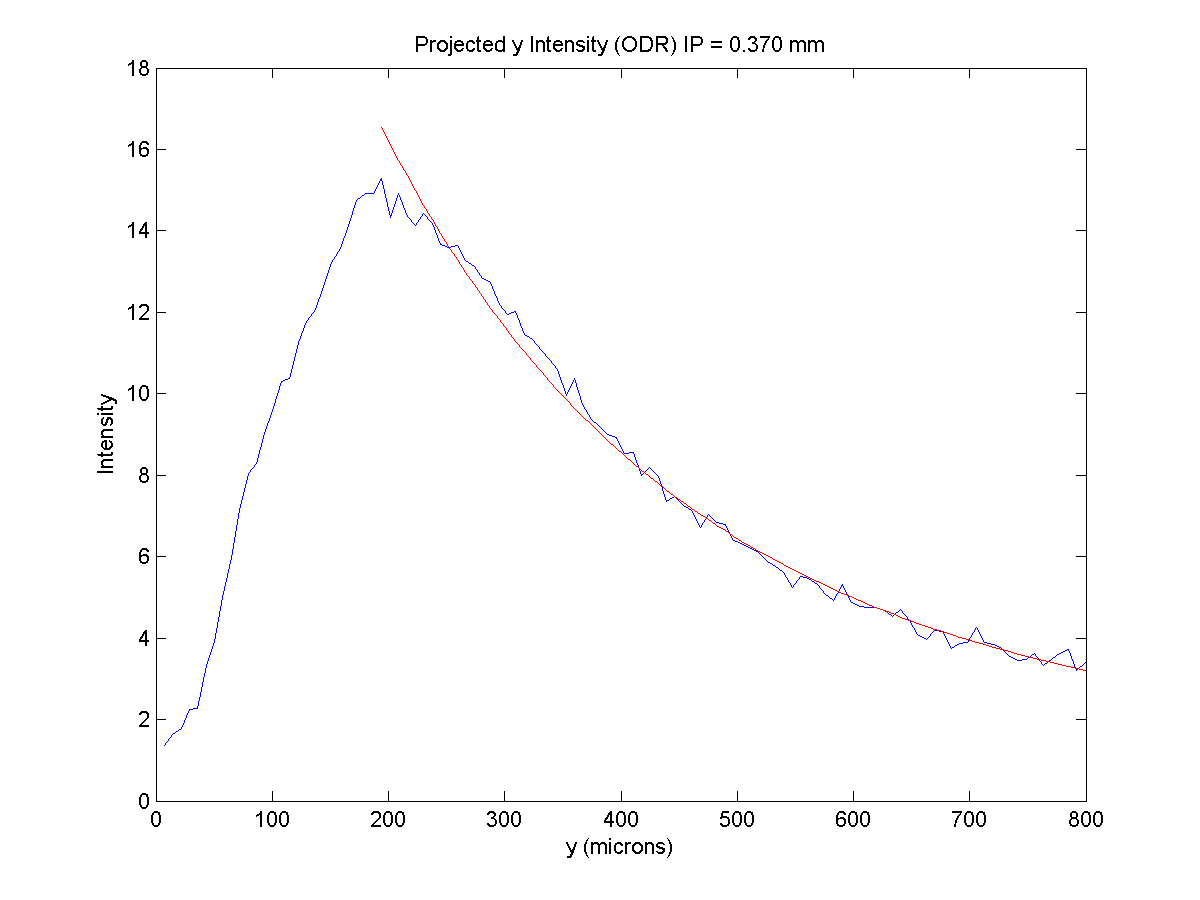
\includegraphics[scale=0.5]{Figures/ProjY_ODR_370.PNG}
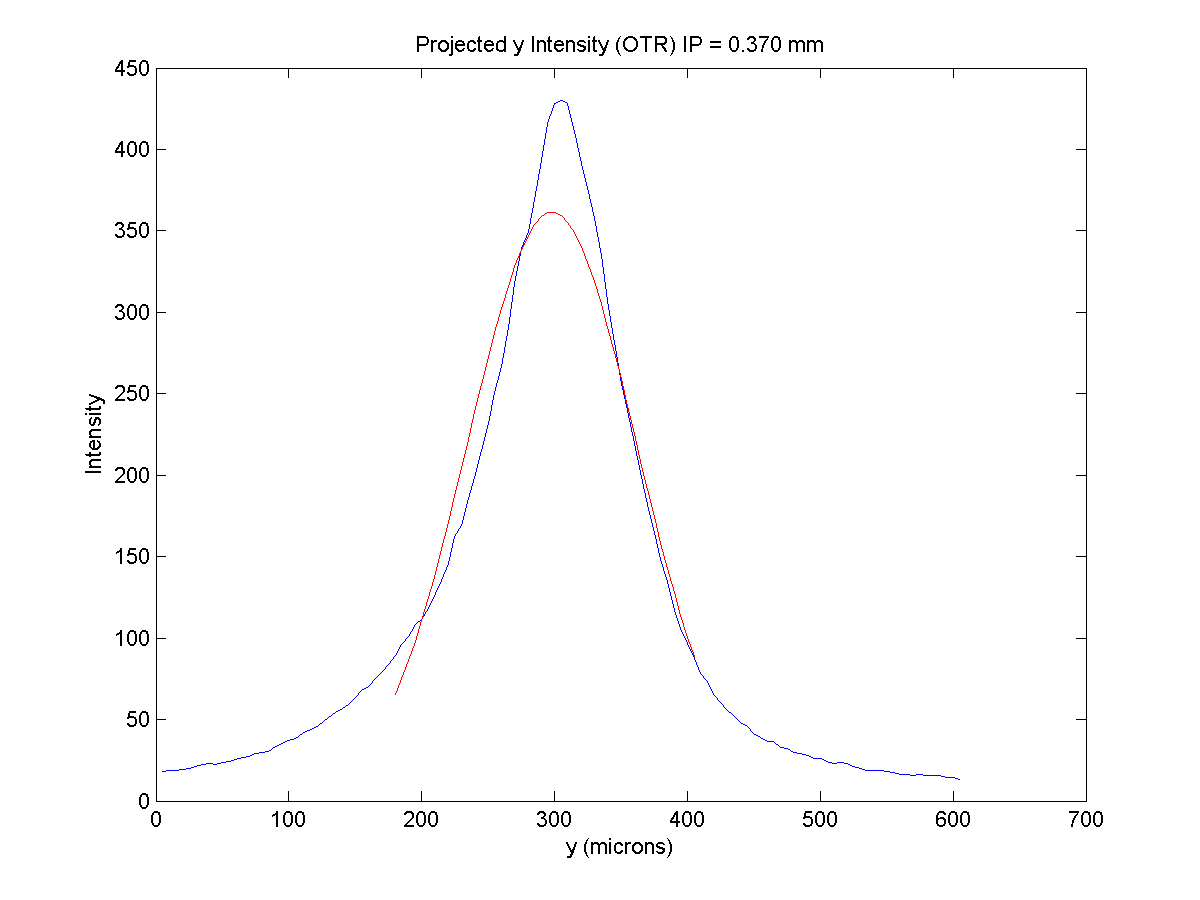
\includegraphics[scale=0.5]{Figures/ProjY_OTR_370.PNG}
\caption{}
\end{center}
\end{figure}

\begin{figure}
\begin{center}
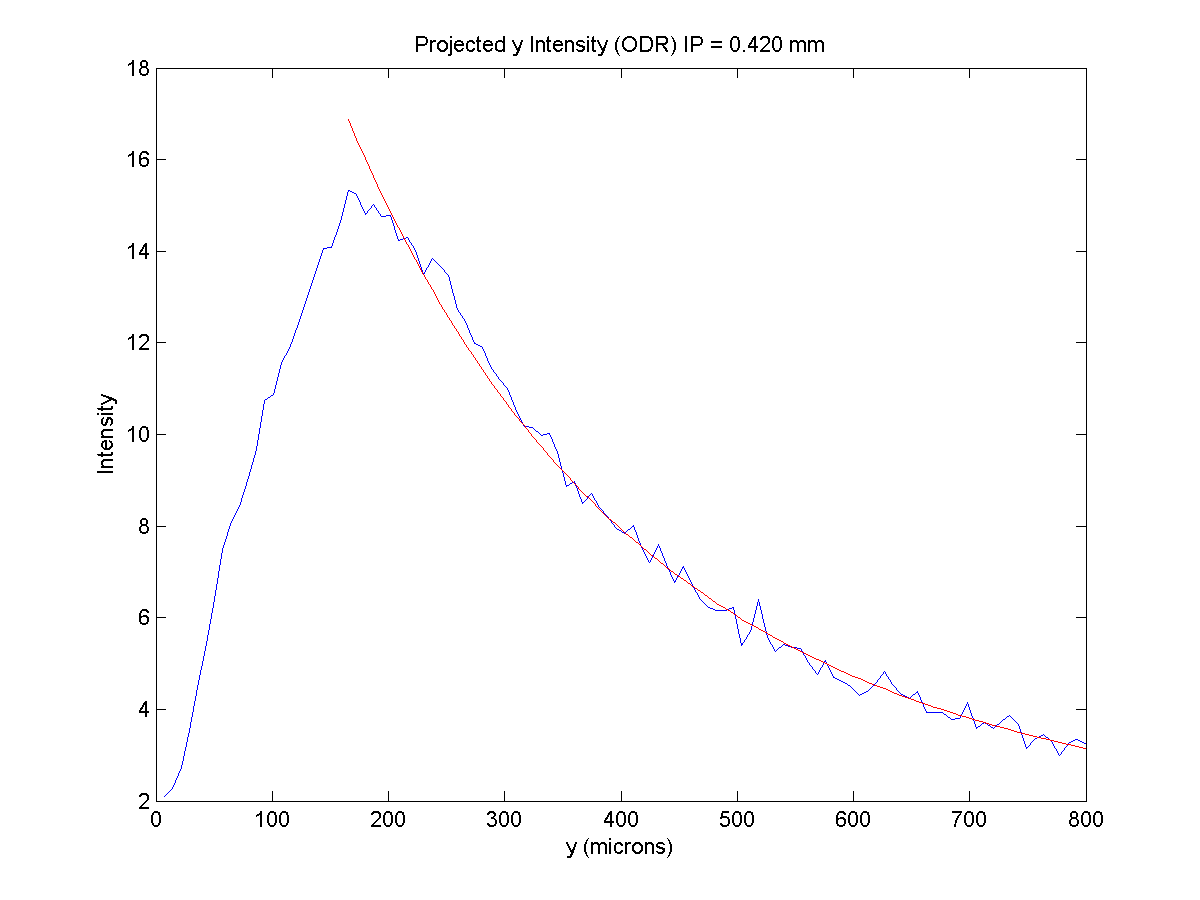
\includegraphics[scale=0.5]{Figures/ProjY_ODR_420.PNG}
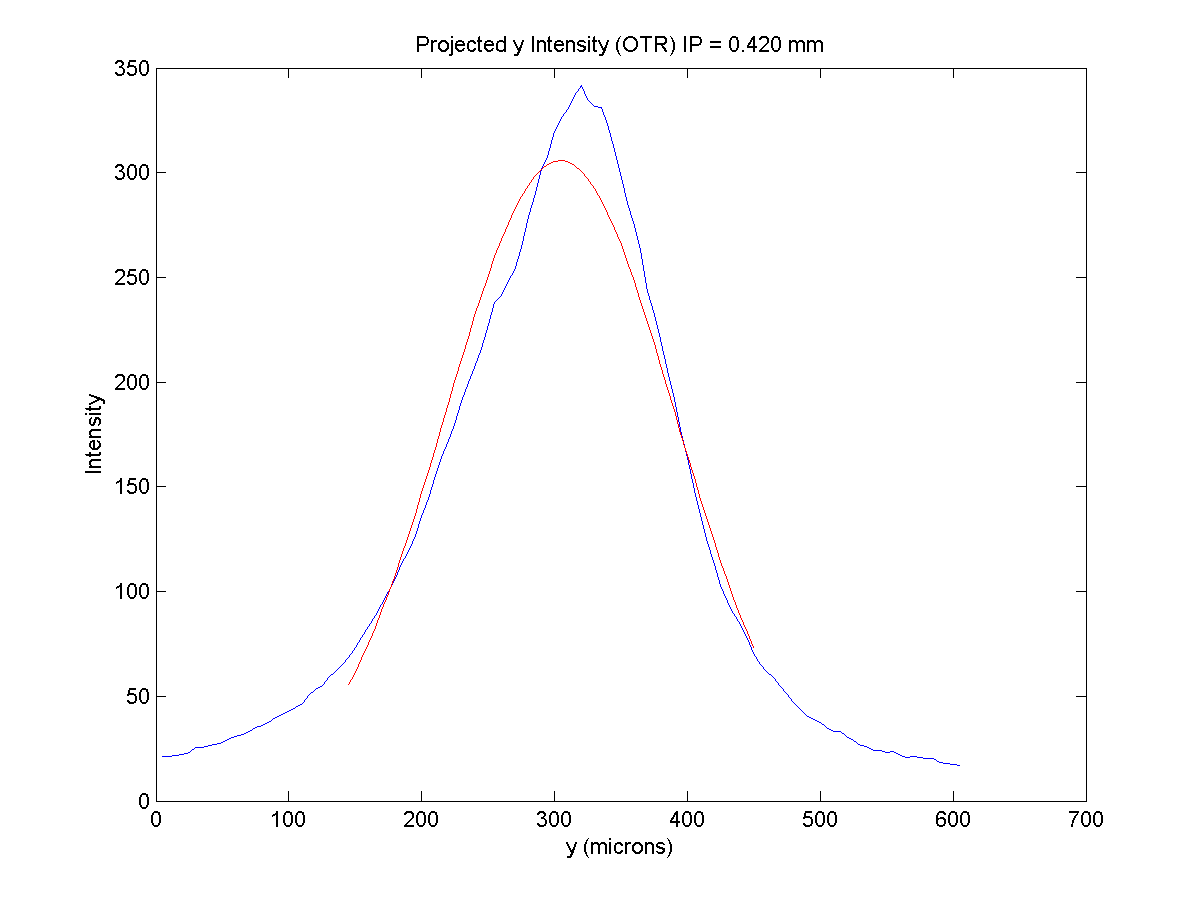
\includegraphics[scale=0.5]{Figures/ProjY_OTR_420.PNG}
\caption{}
\end{center}
\end{figure}

\begin{figure}
\begin{center}
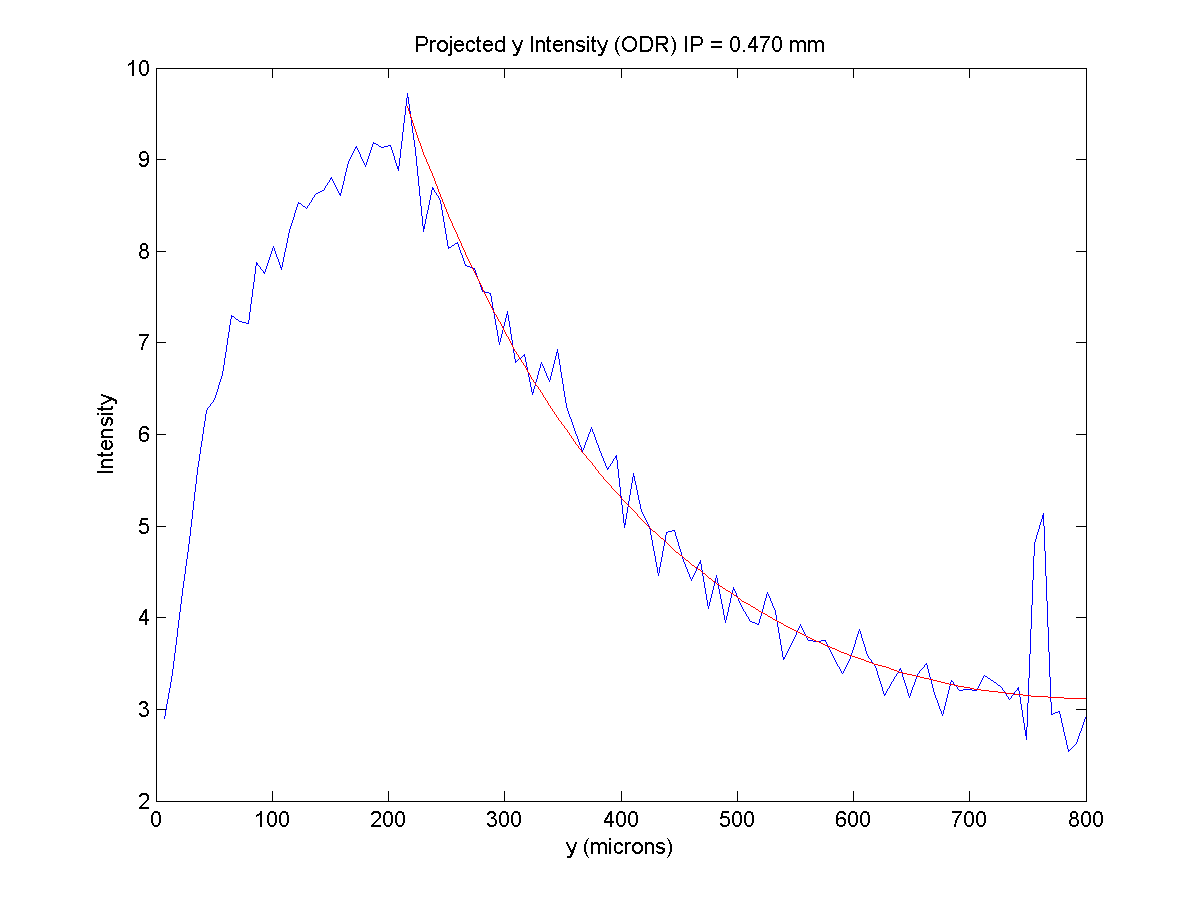
\includegraphics[scale=0.5]{Figures/ProjY_ODR_470.PNG}
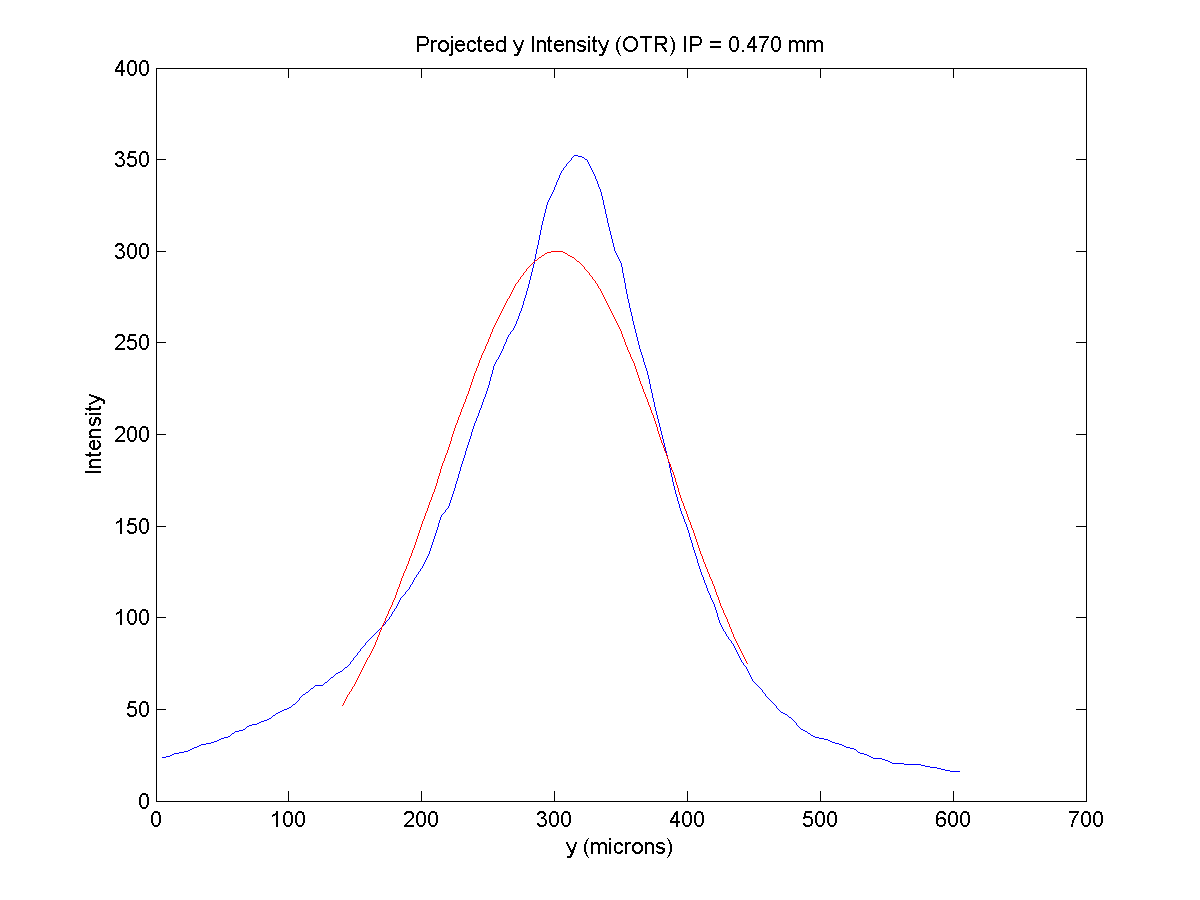
\includegraphics[scale=0.5]{Figures/ProjY_OTR_470.PNG}
\caption{}
\end{center}
\end{figure}

\begin{figure}
\begin{center}
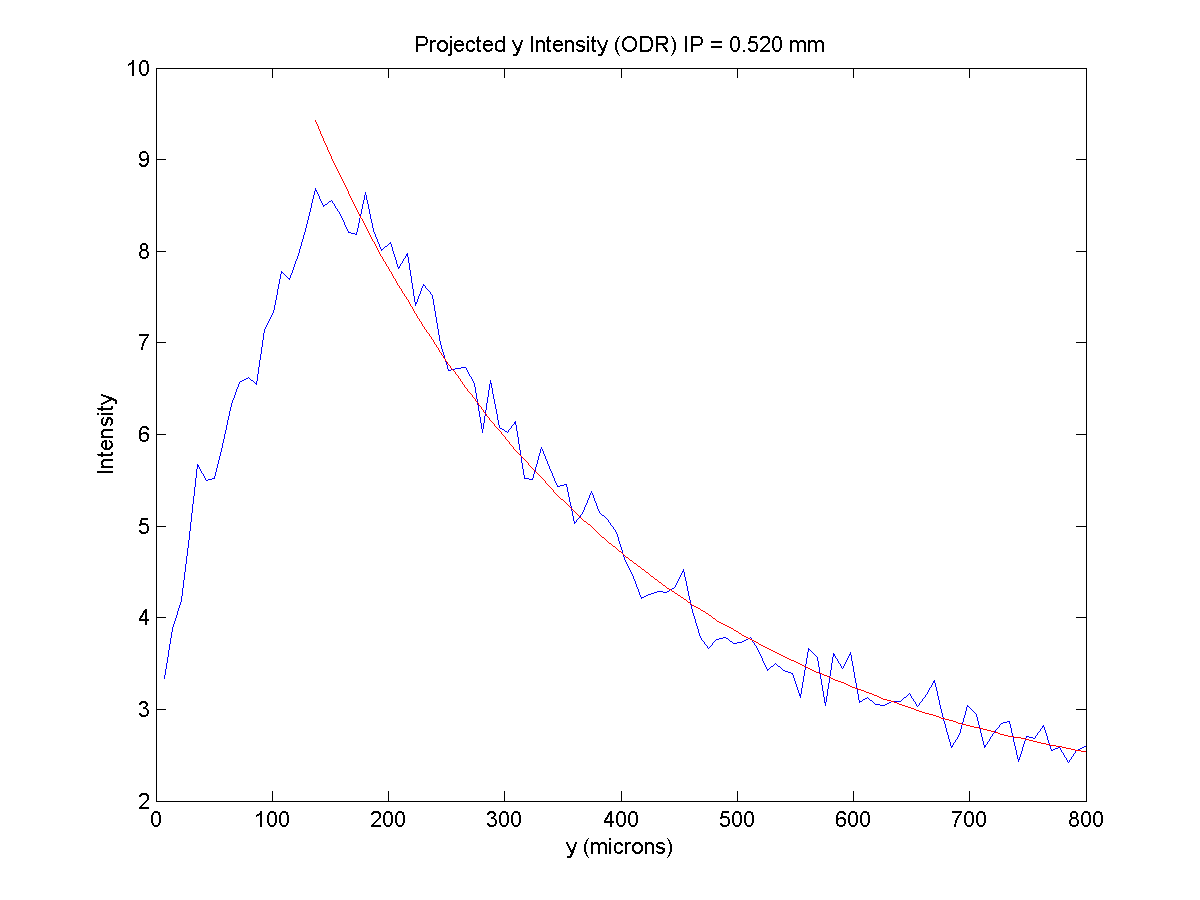
\includegraphics[scale=0.5]{Figures/ProjY_ODR_520.PNG}
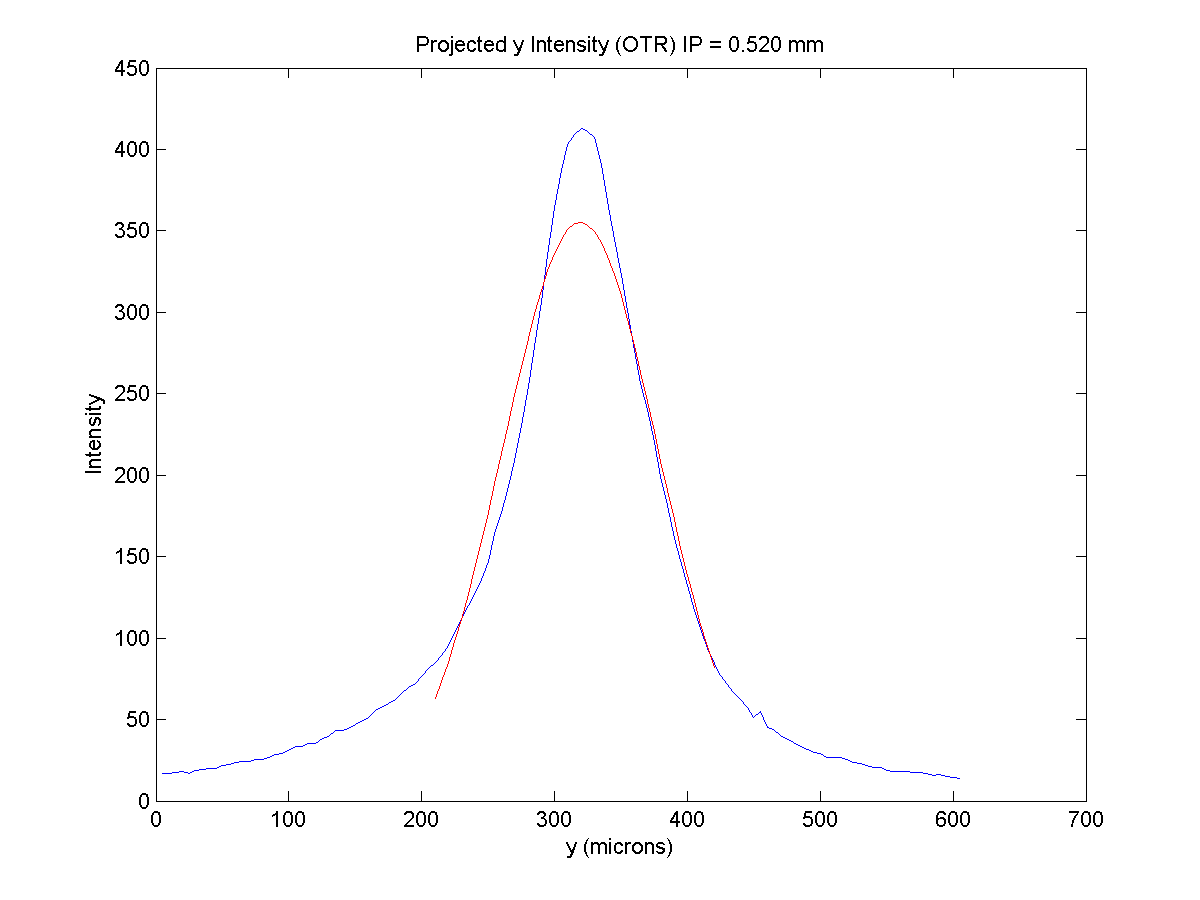
\includegraphics[scale=0.5]{Figures/ProjY_OTR_520.PNG}
\caption{}
\end{center}
\end{figure}

\begin{figure}
\begin{center}
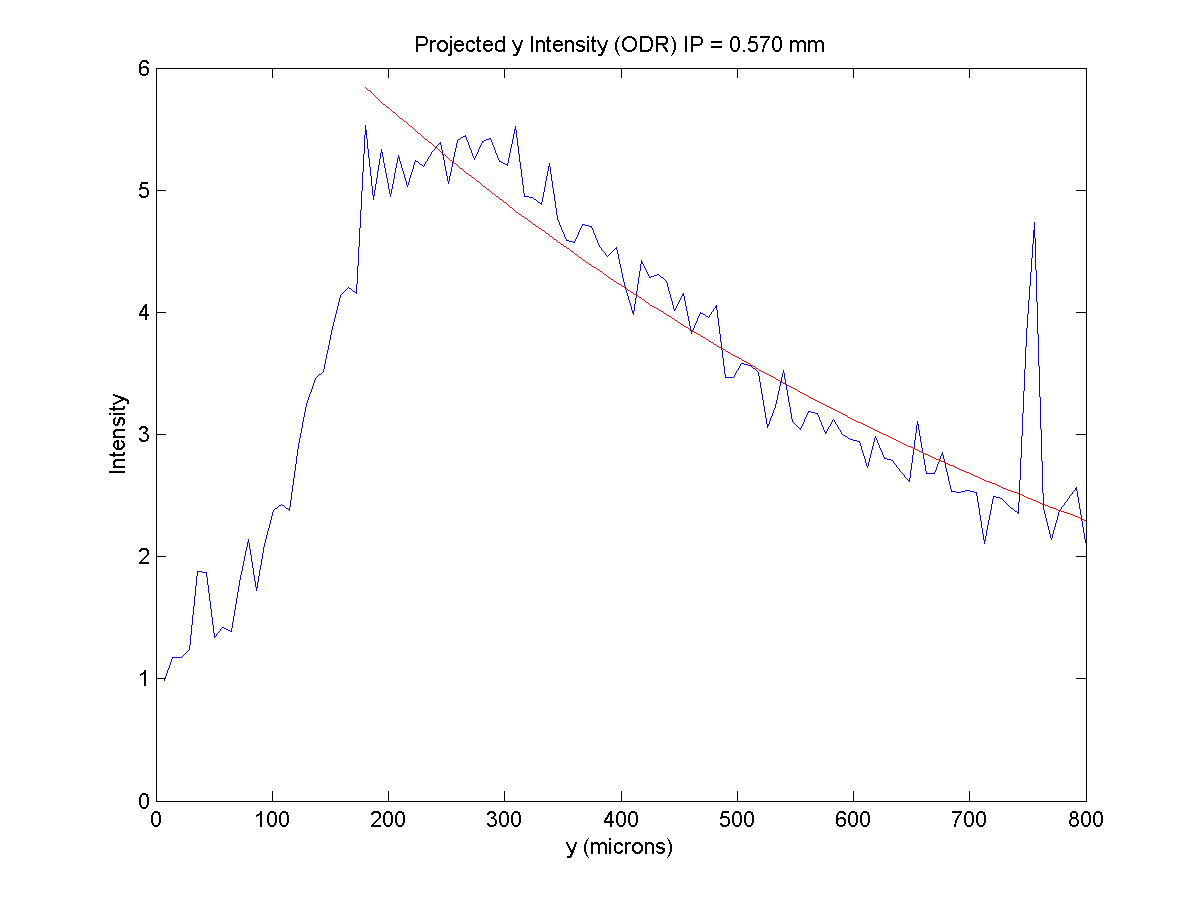
\includegraphics[scale=0.5]{Figures/ProjY_ODR_570.PNG}
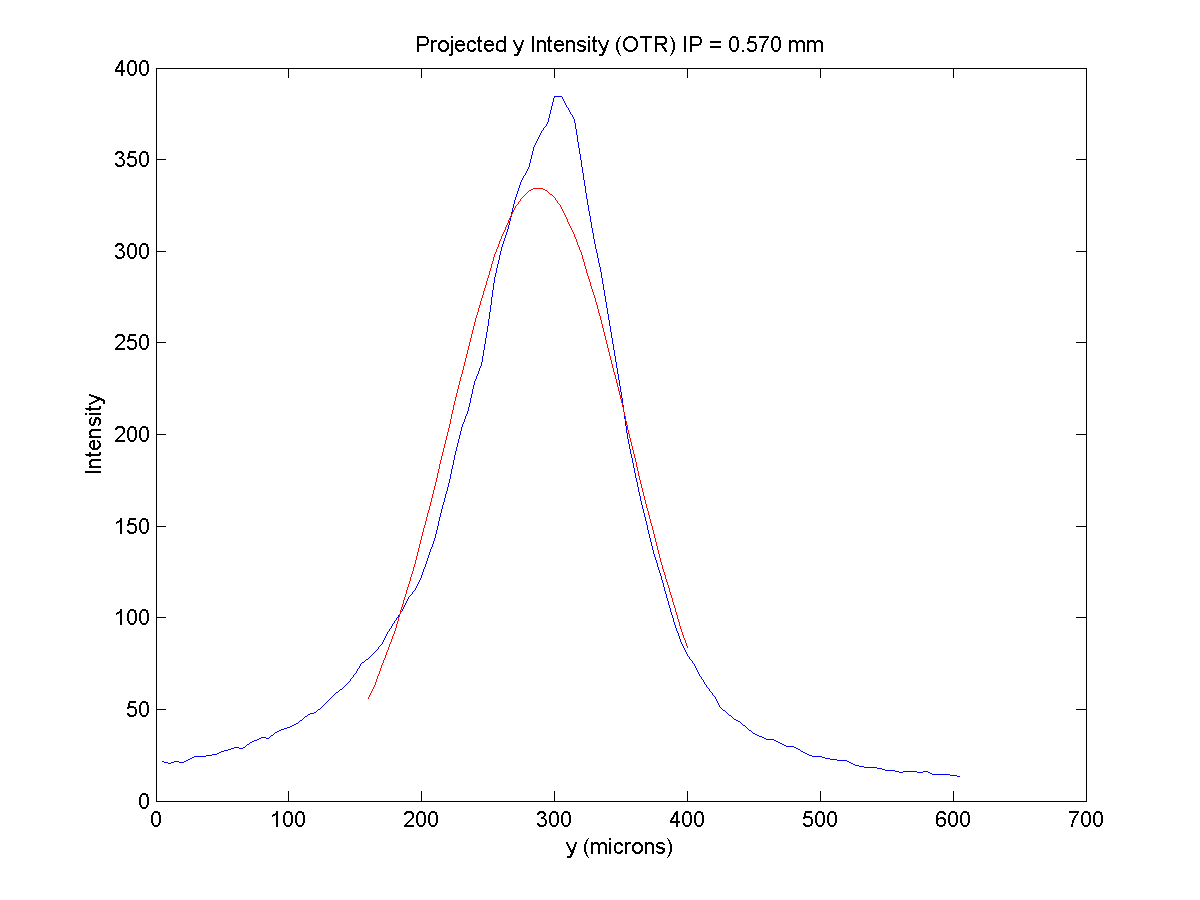
\includegraphics[scale=0.5]{Figures/ProjY_OTR_570.PNG}
\caption{}
\end{center}
\end{figure}



\newpage

\section{Waterfall Projected X Intensity}

These figures show the waterfall plots for the projected X intensity for ODR and OTR for each shot for 500 shots total.

\begin{figure}
\begin{center}
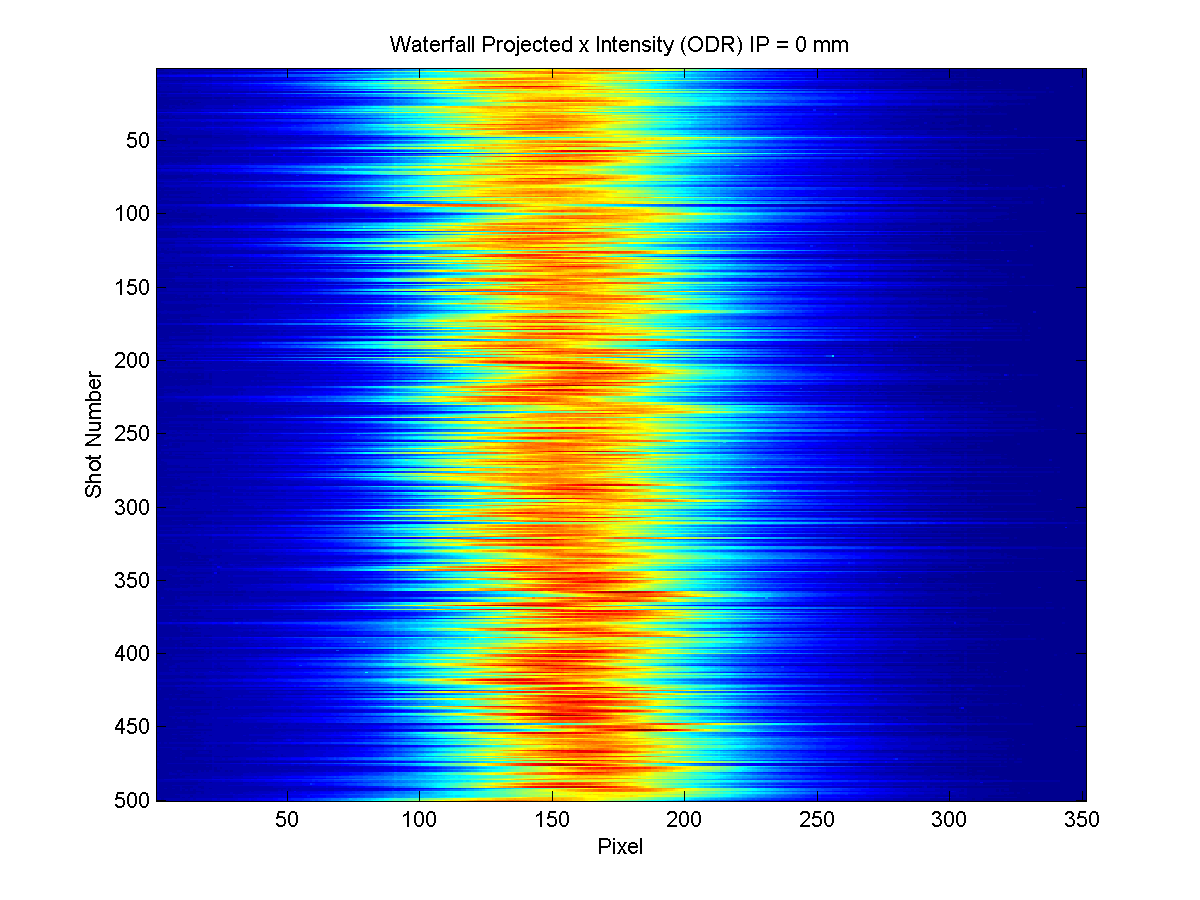
\includegraphics[scale=0.5]{Figures/ProjX_wfall_ODR_0.PNG}
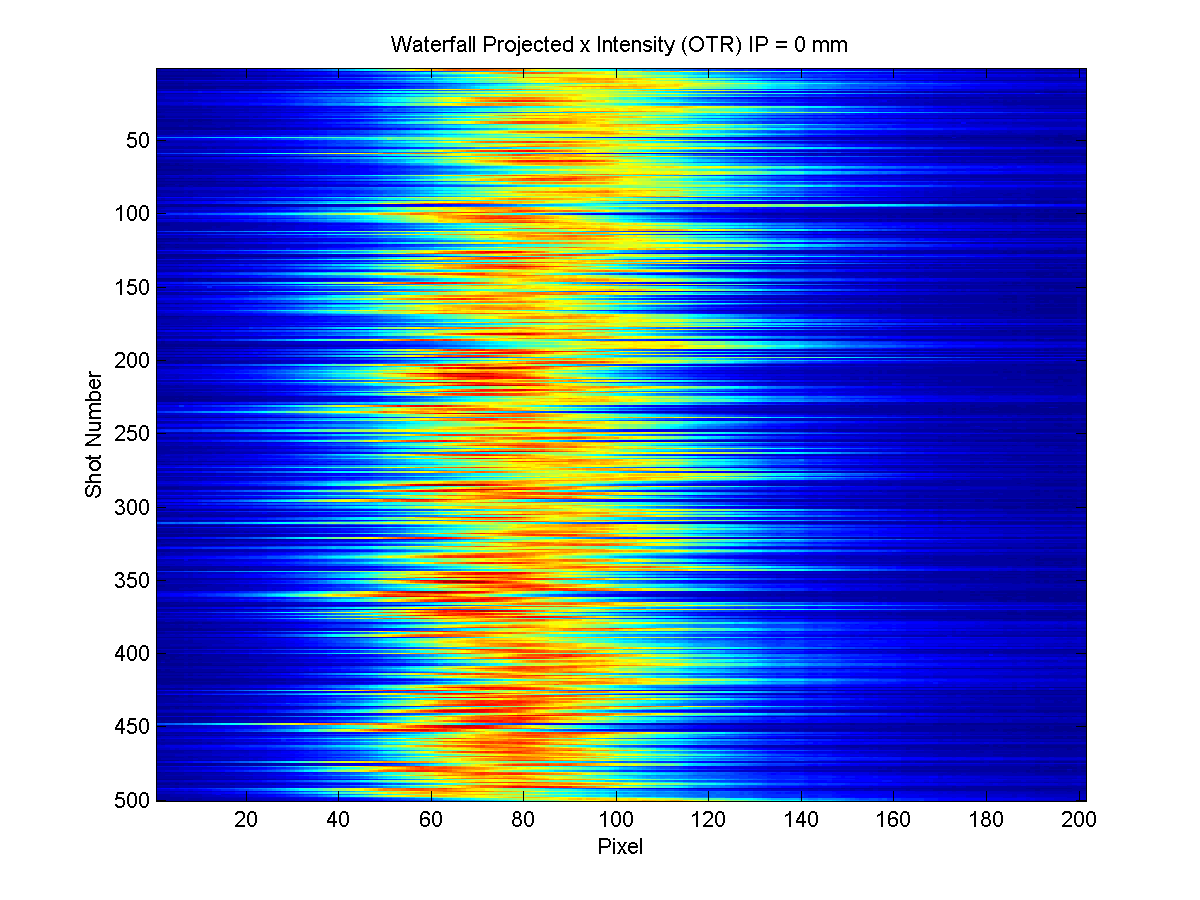
\includegraphics[scale=0.5]{Figures/ProjX_wfall_OTR_0.PNG}
\caption{}
\end{center}
\end{figure}

\begin{figure}
\begin{center}
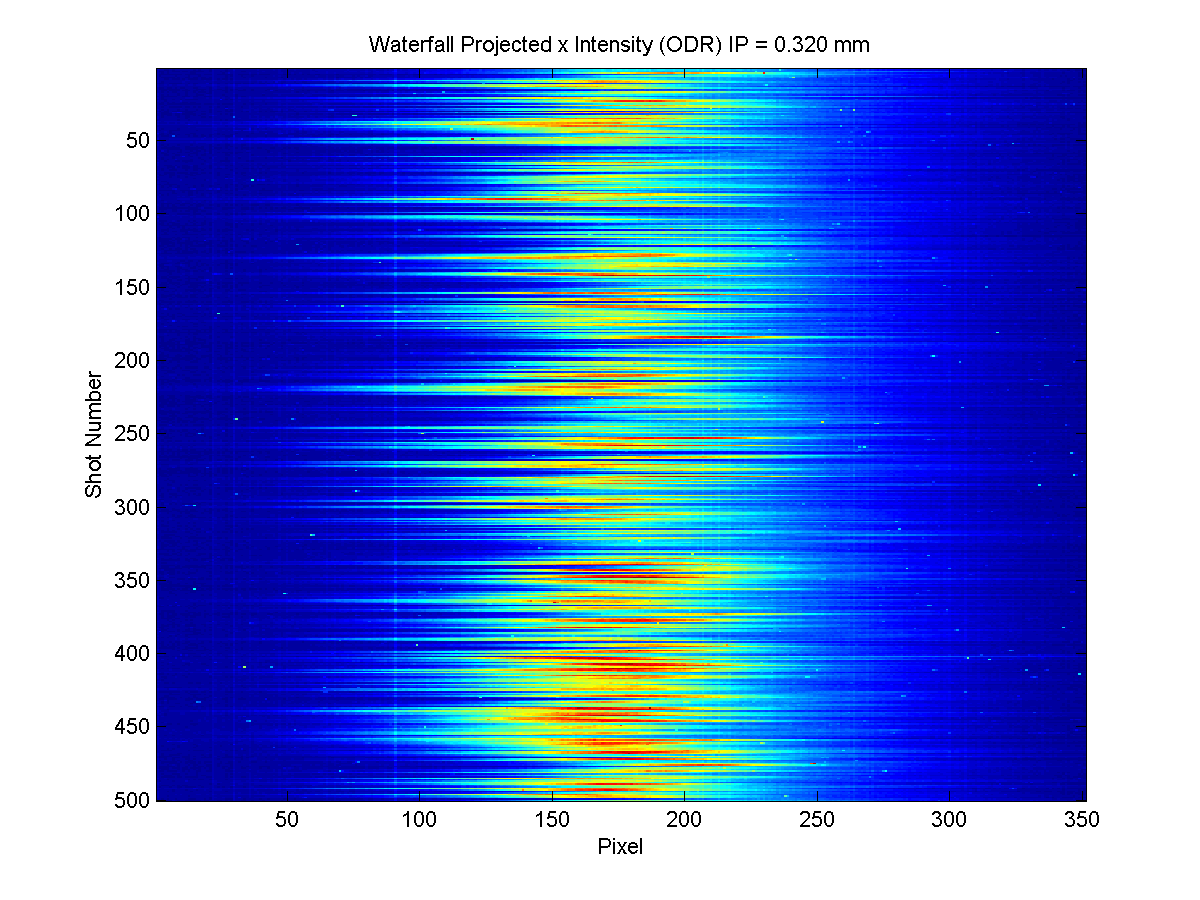
\includegraphics[scale=0.5]{Figures/ProjX_wfall_ODR_320.PNG}
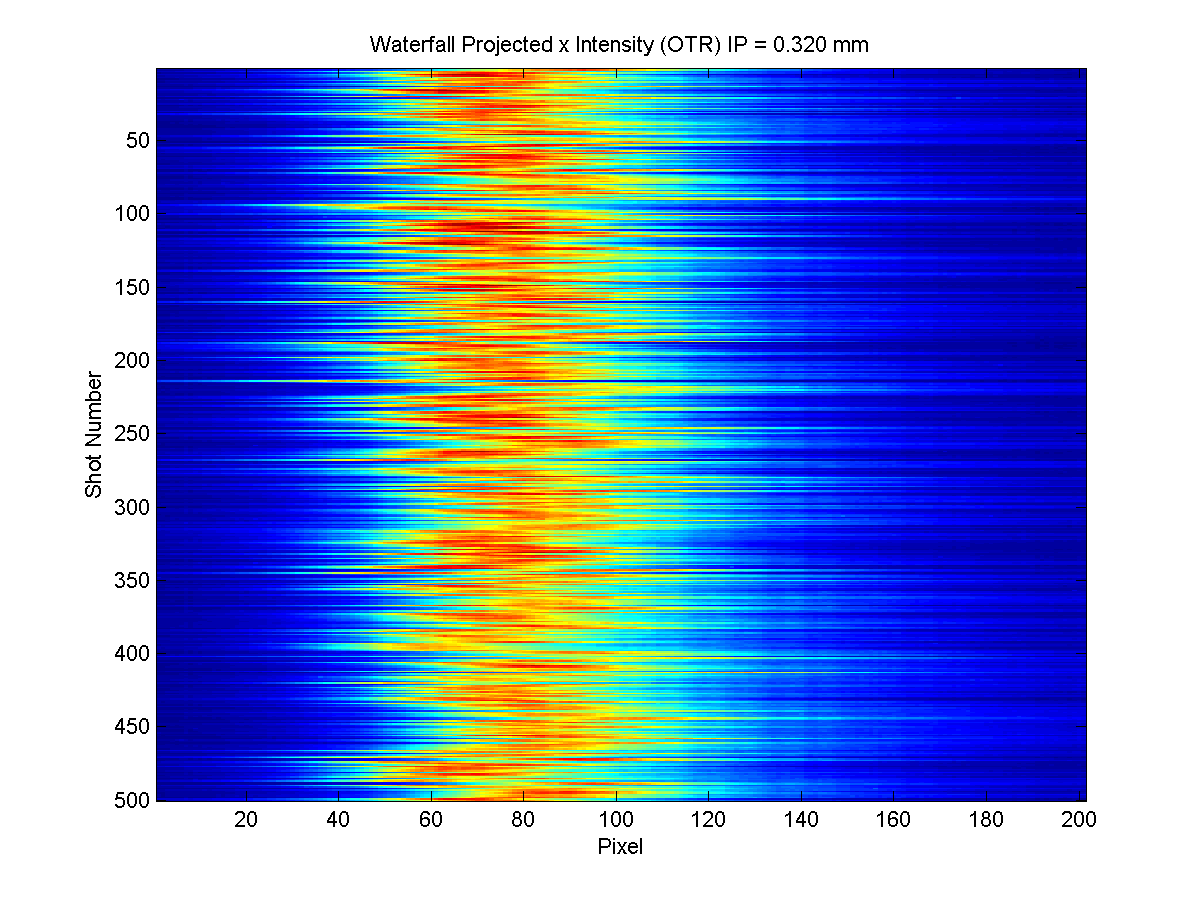
\includegraphics[scale=0.5]{Figures/ProjX_wfall_OTR_320.PNG}
\caption{}
\end{center}
\end{figure}

\begin{figure}
\begin{center}
\includegraphics[scale=0.5]{Figures/ProjX_wfall_ODR_370.PNG}
\includegraphics[scale=0.5]{Figures/ProjX_wfall_OTR_370.PNG}
\caption{}
\end{center}
\end{figure}

\begin{figure}
\begin{center}
\includegraphics[scale=0.5]{Figures/ProjX_wfall_ODR_420.PNG}
\includegraphics[scale=0.5]{Figures/ProjX_wfall_OTR_420.PNG}
\caption{}
\end{center}
\end{figure}

\begin{figure}
\begin{center}
\includegraphics[scale=0.5]{Figures/ProjX_wfall_ODR_470.PNG}
\includegraphics[scale=0.5]{Figures/ProjX_wfall_OTR_470.PNG}
\caption{}
\end{center}
\end{figure}

\begin{figure}
\begin{center}
\includegraphics[scale=0.5]{Figures/ProjX_wfall_ODR_520.PNG}
\includegraphics[scale=0.5]{Figures/ProjX_wfall_OTR_520.PNG}
\caption{}
\end{center}
\end{figure}

\begin{figure}
\begin{center}
\includegraphics[scale=0.5]{Figures/ProjX_wfall_ODR_570.PNG}
\includegraphics[scale=0.5]{Figures/ProjX_wfall_OTR_570.PNG}
\caption{}
\end{center}
\end{figure}



\newpage

\section{Waterfall Projected Y Intensity}

These figures show the waterfall plots for the projected Y intensity for ODR and OTR for each shot for 500 shots total.

\begin{figure}
\begin{center}
\includegraphics[scale=0.5]{Figures/ProjY_wfall_ODR_0.PNG}
\includegraphics[scale=0.5]{Figures/ProjY_wfall_OTR_0.PNG}
\caption{}
\end{center}
\end{figure}

\begin{figure}
\begin{center}
\includegraphics[scale=0.5]{Figures/ProjY_wfall_ODR_320.PNG}
\includegraphics[scale=0.5]{Figures/ProjY_wfall_OTR_320.PNG}
\caption{}
\end{center}
\end{figure}

\begin{figure}
\begin{center}
\includegraphics[scale=0.5]{Figures/ProjY_wfall_ODR_370.PNG}
\includegraphics[scale=0.5]{Figures/ProjY_wfall_OTR_370.PNG}
\caption{}
\end{center}
\end{figure}

\begin{figure}
\begin{center}
\includegraphics[scale=0.5]{Figures/ProjY_wfall_ODR_420.PNG}
\includegraphics[scale=0.5]{Figures/ProjY_wfall_OTR_420.PNG}
\caption{}
\end{center}
\end{figure}

\begin{figure}
\begin{center}
\includegraphics[scale=0.5]{Figures/ProjY_wfall_ODR_470.PNG}
\includegraphics[scale=0.5]{Figures/ProjY_wfall_OTR_470.PNG}
\caption{}
\end{center}
\end{figure}

\begin{figure}
\begin{center}
\includegraphics[scale=0.5]{Figures/ProjY_wfall_ODR_520.PNG}
\includegraphics[scale=0.5]{Figures/ProjY_wfall_OTR_520.PNG}
\caption{}
\end{center}
\end{figure}

\begin{figure}
\begin{center}
\includegraphics[scale=0.5]{Figures/ProjY_wfall_ODR_570.PNG}
\includegraphics[scale=0.5]{Figures/ProjY_wfall_OTR_570.PNG}
\caption{}
\end{center}
\end{figure}



\newpage

\section{Sample Images}

These figures show sample images for ODR and OTR for a single shot.

\begin{figure}
\begin{center}
\includegraphics[scale=0.5]{Figures/Sample_ODR_0.PNG}
\includegraphics[scale=0.5]{Figures/Sample_OTR_0.PNG}
\caption{}
\end{center}
\end{figure}

\begin{figure}
\begin{center}
\includegraphics[scale=0.5]{Figures/Sample_ODR_320.PNG}
\includegraphics[scale=0.5]{Figures/Sample_OTR_320.PNG}
\caption{}
\end{center}
\end{figure}

\begin{figure}
\begin{center}
\includegraphics[scale=0.5]{Figures/Sample_ODR_370.PNG}
\includegraphics[scale=0.5]{Figures/Sample_OTR_370.PNG}
\caption{}
\end{center}
\end{figure}

\begin{figure}
\begin{center}
\includegraphics[scale=0.5]{Figures/Sample_ODR_420.PNG}
\includegraphics[scale=0.5]{Figures/Sample_OTR_420.PNG}
\caption{}
\end{center}
\end{figure}

\begin{figure}
\begin{center}
\includegraphics[scale=0.5]{Figures/Sample_ODR_470.PNG}
\includegraphics[scale=0.5]{Figures/Sample_OTR_470.PNG}
\caption{}
\end{center}
\end{figure}

\begin{figure}
\begin{center}
\includegraphics[scale=0.5]{Figures/Sample_ODR_520.PNG}
\includegraphics[scale=0.5]{Figures/Sample_OTR_520.PNG}
\caption{}
\end{center}
\end{figure}

\begin{figure}
\begin{center}
\includegraphics[scale=0.5]{Figures/Sample_ODR_570.PNG}
\includegraphics[scale=0.5]{Figures/Sample_OTR_570.PNG}
\caption{}
\end{center}
\end{figure}



\newpage

\section{Beam Image Widths}

These figures show the beam image widths for ODR and OTR for each shot for 500 shots total.

\begin{figure}
\begin{center}
\includegraphics[scale=0.5]{Figures/ImageWidth_ODR_0.PNG}
\includegraphics[scale=0.5]{Figures/ImageWidth_OTR_0.PNG}
\caption{}
\end{center}
\end{figure}

\begin{figure}
\begin{center}
\includegraphics[scale=0.5]{Figures/ImageWidth_ODR_320.PNG}
\includegraphics[scale=0.5]{Figures/ImageWidth_OTR_320.PNG}
\caption{}
\end{center}
\end{figure}

\begin{figure}
\begin{center}
\includegraphics[scale=0.5]{Figures/ImageWidth_ODR_370.PNG}
\includegraphics[scale=0.5]{Figures/ImageWidth_OTR_370.PNG}
\caption{}
\end{center}
\end{figure}

\begin{figure}
\begin{center}
\includegraphics[scale=0.5]{Figures/ImageWidth_ODR_420.PNG}
\includegraphics[scale=0.5]{Figures/ImageWidth_OTR_420.PNG}
\caption{}
\end{center}
\end{figure}

\begin{figure}
\begin{center}
\includegraphics[scale=0.5]{Figures/ImageWidth_ODR_470.PNG}
\includegraphics[scale=0.5]{Figures/ImageWidth_OTR_470.PNG}
\caption{}
\end{center}
\end{figure}

\begin{figure}
\begin{center}
\includegraphics[scale=0.5]{Figures/ImageWidth_ODR_520.PNG}
\includegraphics[scale=0.5]{Figures/ImageWidth_OTR_520.PNG}
\caption{}
\end{center}
\end{figure}

\begin{figure}
\begin{center}
\includegraphics[scale=0.5]{Figures/ImageWidth_ODR_570.PNG}
\includegraphics[scale=0.5]{Figures/ImageWidth_OTR_570.PNG}
\caption{}
\end{center}
\end{figure}



\newpage

\section{Beam Image Widths Correlated}

These figures attempt to correlated the beam image widths for ODR and OTR for each shot for 500 shots total.

\begin{figure}
\begin{center}
\includegraphics[scale=0.5]{Figures/ImageWidth_OTRODR_0.PNG}
\caption{}
\end{center}
\end{figure}

\begin{figure}
\begin{center}
\includegraphics[scale=0.5]{Figures/ImageWidth_OTRODR_320.PNG}
\caption{}
\end{center}
\end{figure}

\begin{figure}
\begin{center}
\includegraphics[scale=0.5]{Figures/ImageWidth_OTRODR_370.PNG}
\caption{}
\end{center}
\end{figure}

\begin{figure}
\begin{center}
\includegraphics[scale=0.5]{Figures/ImageWidth_OTRODR_420.PNG}
\caption{}
\end{center}
\end{figure}

\begin{figure}
\begin{center}
\includegraphics[scale=0.5]{Figures/ImageWidth_OTRODR_470.PNG}
\caption{}
\end{center}
\end{figure}

\begin{figure}
\begin{center}
\includegraphics[scale=0.5]{Figures/ImageWidth_OTRODR_520.PNG}
\caption{}
\end{center}
\end{figure}

\begin{figure}
\begin{center}
\includegraphics[scale=0.5]{Figures/ImageWidth_OTRODR_570.PNG}
\caption{}
\end{center}
\end{figure}




\newpage

\section{Beam Image X Position Correlation}

These figures attempt to correlated the beamcentroid x positions for ODR and OTR for each shot for 500 shots total.

\begin{figure}
\begin{center}
\includegraphics[scale=0.5]{Figures/XPosition_OTRODR_0.PNG}
\caption{}
\end{center}
\end{figure}

\begin{figure}
\begin{center}
\includegraphics[scale=0.5]{Figures/XPosition_OTRODR_320.PNG}
\caption{}
\end{center}
\end{figure}

\begin{figure}
\begin{center}
\includegraphics[scale=0.5]{Figures/XPosition_OTRODR_370.PNG}
\caption{}
\end{center}
\end{figure}

\begin{figure}
\begin{center}
\includegraphics[scale=0.5]{Figures/XPosition_OTRODR_420.PNG}
\caption{}
\end{center}
\end{figure}

\begin{figure}
\begin{center}
\includegraphics[scale=0.5]{Figures/XPosition_OTRODR_470.PNG}
\caption{}
\end{center}
\end{figure}

\begin{figure}
\begin{center}
\includegraphics[scale=0.5]{Figures/XPosition_OTRODR_520.PNG}
\caption{}
\end{center}
\end{figure}

\begin{figure}
\begin{center}
\includegraphics[scale=0.5]{Figures/XPosition_OTRODR_570.PNG}
\caption{}
\end{center}
\end{figure}


\newpage

\section{Beam Image Y Position Correlation}

These figures attempt to correlated the beamcentroid y positions for ODR and OTR for each shot for 500 shots total.

\begin{figure}
\begin{center}
\includegraphics[scale=0.5]{Figures/YPosition_OTRODR_0.PNG}
\caption{}
\end{center}
\end{figure}

\begin{figure}
\begin{center}
\includegraphics[scale=0.5]{Figures/YPosition_OTRODR_320.PNG}
\caption{}
\end{center}
\end{figure}

\begin{figure}
\begin{center}
\includegraphics[scale=0.5]{Figures/YPosition_OTRODR_370.PNG}
\caption{}
\end{center}
\end{figure}

\begin{figure}
\begin{center}
\includegraphics[scale=0.5]{Figures/YPosition_OTRODR_420.PNG}
\caption{}
\end{center}
\end{figure}

\begin{figure}
\begin{center}
\includegraphics[scale=0.5]{Figures/YPosition_OTRODR_470.PNG}
\caption{}
\end{center}
\end{figure}

\begin{figure}
\begin{center}
\includegraphics[scale=0.5]{Figures/YPosition_OTRODR_520.PNG}
\caption{}
\end{center}
\end{figure}

\begin{figure}
\begin{center}
\includegraphics[scale=0.5]{Figures/YPosition_OTRODR_570.PNG}
\caption{}
\end{center}
\end{figure}


\newpage

\section{FFT Beam Width}

These figures show the FFT for the beam size as measured by OTR for 500 shots total.

\begin{figure}
\begin{center}
\includegraphics[scale=0.5]{Figures/FFT_0.PNG}
\caption{}
\end{center}
\end{figure}

\begin{figure}
\begin{center}
\includegraphics[scale=0.5]{Figures/FFT_320.PNG}
\caption{}
\end{center}
\end{figure}

\begin{figure}
\begin{center}
\includegraphics[scale=0.5]{Figures/FFT_370.PNG}
\caption{}
\end{center}
\end{figure}

\begin{figure}
\begin{center}
\includegraphics[scale=0.5]{Figures/FFT_420.PNG}
\caption{}
\end{center}
\end{figure}

\begin{figure}
\begin{center}
\includegraphics[scale=0.5]{Figures/FFT_470.PNG}
\caption{}
\end{center}
\end{figure}

\begin{figure}
\begin{center}
\includegraphics[scale=0.5]{Figures/FFT_520.PNG}
\caption{}
\end{center}
\end{figure}

\begin{figure}
\begin{center}
\includegraphics[scale=0.5]{Figures/FFT_570.PNG}
\caption{}
\end{center}
\end{figure}




\end{document}
